\documentclass[11pt,a4paper,hidelinks]{article}

\setlength{\headheight}{26pt}

% Packages
\usepackage[left=25mm, right=25mm, top=35mm, bottom=25mm]{geometry} % defines whitespaces on the edges
\usepackage[bottom, hang]{footmisc}
\usepackage{hyperref}             % for \nameref and cite
\usepackage{footnotebackref}      % used for getting back from the footnote to the main text
\usepackage{enumitem}
\usepackage{graphicx}
\usepackage{fancyhdr}
\usepackage{lastpage}
\usepackage[export]{adjustbox}
\usepackage{float}
\usepackage[ngerman]{babel}
\usepackage[ngerman]{datetime}
\usepackage{apacite}
\usepackage[utf8]{inputenc}
\usepackage{listings}
\usepackage{xcolor}
\usepackage{pdfpages}
\usepackage{url}
\usepackage{outlines}
\usepackage{tocloft}
\usepackage[utf8]{inputenc}
\usepackage{amsmath}
\usepackage{mathtools}
\usepackage[acronym]{glossaries}
\usepackage{titlesec}             % for \titleformat
\usepackage{textcomp}             % for \degree sign
\usepackage{gensymb}              % for \degree sign
\usepackage{csvsimple}            % for using csv-files for tables
\usepackage{lscape}               % for landscape mode
\usepackage{parskip}              % inserts space after paragraph automatically
\usepackage{svg}                  % used to include svg with the help of inkscape which converts svg to pdf
\usepackage{wasysym}              % for \diameter symbol
\usepackage{xfrac}                % for \sfrac

\frenchspacing  % Use same space size between words and between sentences

% change section titles' font size
\titleformat*{\section}{\huge\bfseries}
\titleformat*{\subsection}{\LARGE\bfseries}
\titleformat*{\subsubsection}{\Large\bfseries}
\titleformat{\paragraph}[hang]{\large\bfseries}{\theparagraph}{1em}{}
\titleformat{\subparagraph}[hang]{\normalsize\bfseries}{\thesubparagraph}{1em}{}

\definecolor{codegreen}{rgb}{0,0.6,0}
\definecolor{codegray}{rgb}{0.5,0.5,0.5}
\definecolor{codepurple}{rgb}{0.58,0,0.82}
\definecolor{codeorange}{rgb}{1,0.5,0.15}
\definecolor{backcolour}{rgb}{0.9,0.9,0.9}

\lstdefinestyle{mystyle}{
    backgroundcolor=\color{backcolour},
    commentstyle=\color{codegreen},
    keywordstyle=\color{magenta},
    numberstyle=\tiny\color{codegray},
    stringstyle=\color{codepurple},
    basicstyle=\ttfamily\footnotesize,
    breakatwhitespace=false,
    breaklines=true,
    captionpos=b,
    keepspaces=true,
    numbers=left,
    numbersep=5pt,
    showspaces=false,
    showstringspaces=false,
    showtabs=false,
    tabsize=4
}
\lstset{style=mystyle}

\lstset{
    literate={~} {$\sim$}{1}
}

\lstset{%
    breaklines=true,
    breakatwhitespace=true,
}

\DeclarePairedDelimiter\abs{\lvert}{\rvert} % make scalable absolute stripes
\DeclarePairedDelimiter\parenth{(}{)} % make scalable parentheses

\let\phi\varphi{} % change style of \phi sign

\setlength{\parindent}{0mm} % disable paragraph indent

\newdateformat{mydate}{\THEDAY{. }\monthnamengerman[\THEMONTH] \THEYEAR}

\renewcommand{\listfigurename}{}
\renewcommand\contentsname{Inhaltsverzeichnis}
\renewcommand\lstlistingname{Code}

\makeglossaries{}

% Header/Footer Setting
\setlength\footnotemargin{15pt}
\pagestyle{fancy}
\fancyhf{}
\renewcommand{\footrulewidth}{0.4pt} % footer line
\rhead{\textbf{\vUniversity}\\\vModule}
\lhead{\textbf{\vTitle}\\
    Projektarbeit}
\lfoot{\vAuthorFirstName{} \vAuthorLastName}
\cfoot{\mydate\today}
\rfoot{S.~\thepage~/~\pageref{LastPage}}

% Redefine the plain page style, otherwise there is no header and footer for chapter pages
\fancypagestyle{plain}{%
    \fancyhf{}
    \renewcommand{\footrulewidth}{0.4pt} % footer line
    \rhead{\textbf{\vUniversity}\\\vModule}
    \lhead{\textbf{\vTitle}\\
        Projektarbeit}
    \lfoot{\vAuthorFirstName{} \vAuthorLastName}
    \cfoot{\mydate\today}
    \rfoot{S.~\thepage~/~\pageref{LastPage}}
}

\bibliographystyle{apacite}

% Settings for the equation list
\newcommand{\listequationsname}{}
\newlistof{myequations}{equ}{\listequationsname}
\renewcommand{\cftmyequationsaftersnum}{\hfill}
\renewcommand{\cftmyequationspresnum}{\hfill}
\setlength{\cftmyequationsnumwidth}{3.5em}
\newcommand{\myequations}[1]{%
\addcontentsline{equ}{myequations}{\protect\numberline{\theequation}#1}\par}

\newcommand{\mytable}[4]
{
    \centering
    \begin{tabular}{#1}\hline%
        #2 \\ \hline
        \csvreader[
            separator=semicolon,
            head to column names,
            late after line=\\,
        ]{#4}{}{#3}
        \hline
    \end{tabular}
}


% Variables
\newcommand{\vTitle}{DIY Optische ToF Distanzmessung}
\newcommand{\vModule}{CAS Sensorik und Sensor Signal Conditioning}
\newcommand{\vAuthorFirstName}{Matthias Schär,}
\newcommand{\vAuthorLastName}{Timon Burkard}
\newcommand{\vUniversity}{OST -- Ostschweizer Fachhochschule}
\newcommand{\vDegree}{CAS Sensorik und Sensor Signal Conditioning}
\newcommand{\vSemester}{HS24}
\newcommand{\vProfessor}{Prof. Guido Keel, Michael Lehmann}
\newcommand{\vCity}{Rapperswil}
\newcommand{\vAbstract}{Die vorliegende Projektarbeit befasst sich mit der Entwicklung eines\dots}

% Acronyms
\newacronym{pcb}{PCB}{Printed Circuit Board}
\newacronym{tof}{ToF}{Time of Flight}
\newacronym{diy}{DIY}{Do It Yourself}
\newacronym{adc}{ADC}{Analog to Digital Converter}
\newacronym{tdc}{TDC}{Time to Digital Converter}
\newacronym{tia}{TIA}{Trans-Impedance Amplifier}
\newacronym{mcu}{MCU}{Microcontroller Unit}
\newacronym{cpu}{CPU}{Central Processing Unit}
\newacronym{hal}{HAL}{Hardware Abstraction Layer}
\newacronym{gpio}{GPIO}{General Purpose Input/Output}
\newacronym{uart}{UART}{Universal Asynchronous Receiver/Transmitter}
\newacronym{dso}{DSO}{Digital Storage Oscilloscope}
\newacronym{spi}{SPI}{Serial Peripheral Interface}
\newacronym{ic}{IC}{Integrated Circuit}
\newacronym{usb}{USB}{Universal Serial Bus}
\newacronym{hsi}{HSI}{High Speed Internal}
\newacronym{pll}{PLL}{Phase-Locked Loop}

\begin{document}

\title{\vspace{-40pt}\begin{huge}\textbf{\vTitle}\end{huge}\\
\ \\ \vModule}
\author{\\\\\textbf{\vAuthorFirstName{} \vAuthorLastName}\\
    \vUniversity{}\\
    \\\\}

\date{\mydate\today}
\maketitle\thispagestyle{empty}  % removes footer from first page

\vspace{35pt}

\begin{figure}[H]
    \centering
    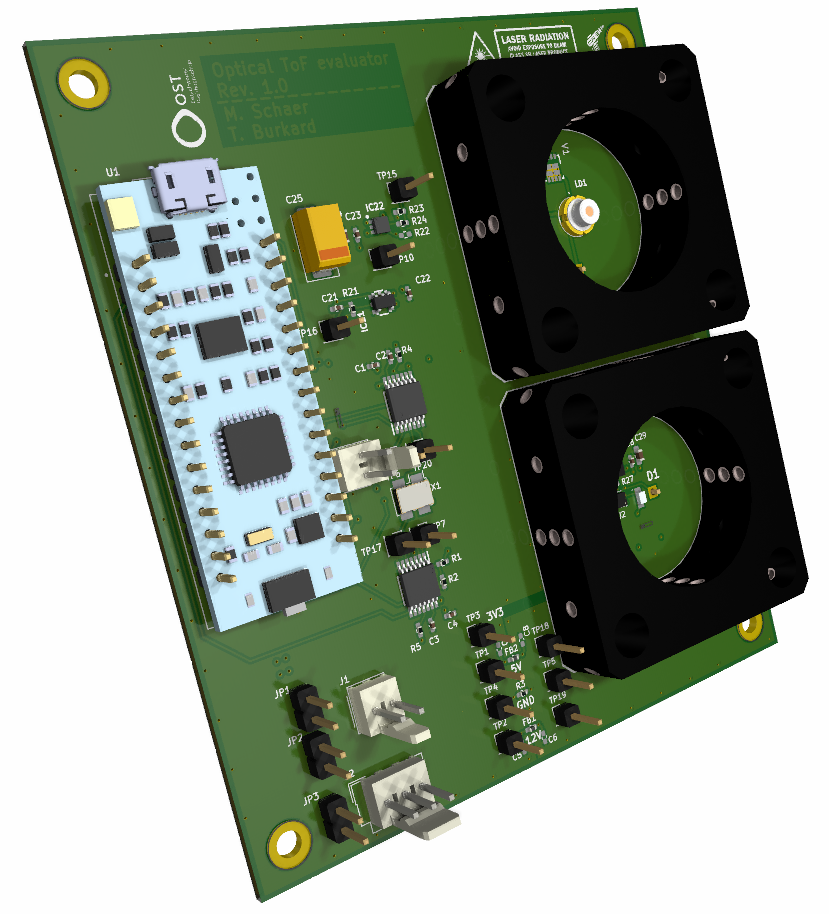
\includegraphics[width=0.6\textwidth]{graphics/cover_picture.png}
\end{figure}

\vspace{30pt}

\begin{figure}[H]
    \centering
    \begin{minipage}[b]{0.3\textwidth}
        \includesvg[width=\textwidth]{graphics/OST_Logo.svg}\label{fig:OST_Logo}
    \end{minipage}
\end{figure}

\pagebreak

\thispagestyle{empty}

\textbf{}
\vspace{5mm}

\begin{flushleft}
    \textbf{\large{\vModule{} an der \vUniversity{}}}
\end{flushleft}

\begin{flushleft}
    \begin{small}
        \begin{tabular}{@{}lll}
            \\
            \textbf{Titel}                 & & \textbf{\vTitle}\\
            \\
            \textbf{Diplomandin/Diplomand} & & \textbf{\vAuthorFirstName{} \vAuthorLastName}\\
            \\
            \textbf{Studiengang}           & & \textbf{\vDegree}\\
            \\
            \textbf{Semester}              & & \textbf{\vSemester}\\
            \\
            \textbf{Dozentin/Dozent}       & & \textbf{\vProfessor}\\
        \end{tabular}
    \end{small}
\end{flushleft}

\vspace{10mm}

% abstracts
\begin{flushleft}
    \begin{small}
        \textbf{Abstract} \\
        \vAbstract{}
        \vspace{15mm}
    \end{small}
\end{flushleft}

% copyright
\begin{flushleft}
    \begin{small}
        Ort, Datum\hspace{30mm}\vCity, \date{\mydate\today} \\
        \textbf{\textcopyright\hspace{1mm}\vAuthorFirstName{} \vAuthorLastName, \vUniversity{}}
    \end{small}
\end{flushleft}

\mbox{}
\vfill

\noindent\makebox[\linewidth]{\rule{\textwidth}{1pt}}
% copyright notice
\begin{flushleft}
    \begin{small}
        Alle Rechte vorbehalten. Die Arbeit oder Teile davon dürfen ohne schriftliche Genehmigung der Rechteinhaber weder in irgendeiner Form reproduziert noch elektronisch gespeichert, verarbeitet, vervielfältigt oder verbreitet werden.\\~\\
        Sofern die Arbeit auf der Website der Ostschweizer Fachhochschule online veröffentlicht wird, können abweichende Nutzungsbedingungen unter Creative-Commons-Lizenzen gelten. Massgebend ist in diesem Fall die auf der Website angezeigte Creative-Commons-Lizenz.
    \end{small}
\end{flushleft}

\pagebreak

\section*{Inhaltsverzeichnis}
\vspace{-25pt}
\renewcommand*\contentsname{}
\tableofcontents

\pagebreak

\section*{Abkürzungsverzeichnis}
\vspace{-25pt}
\printglossary[type=\acronymtype,title={}]

\pagebreak

\section*{Abbildungsverzeichnis}
\vspace{-25pt}
\renewcommand{\listfigurename}{}
\listoffigures

\pagebreak

\section*{Formelverzeichnis}
\vspace{-25pt}
\listofmyequations{}

\pagebreak

\section*{Tabellenverzeichnis}
\vspace{-25pt}
\renewcommand{\listtablename}{}
\listoftables

\pagebreak

\section*{Codeverzeichnis}
\vspace{-33pt}
\renewcommand{\lstlistlistingname}{}
\lstlistoflistings{}

\pagebreak


%%%%%%%%%%%%%%%%%%%%%% CONTENT START %%%%%%%%%%%%%%%%%%%%%%

\section{Einleitung}

Bei dieser Projektarbeit geht es darum ein \acrfull{diy} optisches \acrfull{tof} Distanzmesssystem aufzubauen. Dazu soll
ein \acrfull{tdc} verwendet werden.

\dots

\pagebreak

\section{Theorie}

\subsection{Time of Flight}

Bei \acrshort{tof} handelt es sich um \dots

\pagebreak

\subsection{Photostrom}

Zur Berechnung des theoretisch zu erwartenden Photostrom wird von einer Distanz zur Wand von $10~m$ ausgegangen.

Der Laserstrahl gehe idealisiert mit $0\degree$ zur Wand und werde dort uniform Halbkugel-förmig gestreut. In der
Realität wird sich die Streuung nicht uniform verteilen, sondern in der Mitte stärker konzentriert sein. Die folgende
Berechnung zeigt also den worst case.

Die Berechnung der empfangenen Strahlungsleistung, der Strahlungsintensität, dem Raumwinkel und dem Photostrom sind in
Formel~\ref{eq:pin}, \ref{eq:ie}, \ref{eq:omega} bzw. \ref{eq:iph} gezeigt.

\begin{equation}\label{eq:pin}
    P_{in} = E_e \cdot A = \frac{I_e}{r^2} \cdot A
\end{equation}
\myequations{Eintreffende Lichtleistung}

\begin{equation}\label{eq:ie}
    I_e = \frac{P_{out}}{\Omega}
\end{equation}
\myequations{Strahlungsintensität}

\begin{equation}\label{eq:omega}
    \Omega = \frac{4\cdot \pi \cdot 0.5}{d}
\end{equation}
\myequations{Raumwinkel}

\begin{equation}\label{eq:iph}
    I_{ph} = S \cdot P_{in}
\end{equation}
\myequations{Photostrom}

\subsubsection{Berechnung mit RLD94PZJ5 und BPV23NF}

Ersten Berechnungen wurden mit der Laserdiode RLD94PZJ5 \cite{rohm2020rld94pzj5_datasheet} und der Photodiode BPV23NF
\cite{vishay2024bpv23nf_datasheet} durchgeführt.

Die relevanten Werte aus den Datenblättern sind in Formel~\ref{eq:rld94pzj5_num} und \ref{eq:rbpv23nf_num} aufgelistet.

\begin{equation}\label{eq:rld94pzj5_num}
    P_{out} = 285~mW
\end{equation}
\myequations{Werte des RLD94PZJ5}

\begin{equation}\label{eq:rbpv23nf_num}
    \begin{split}
        A &= 4.4~mm^2\\
        S &= 0.6~\frac{A}{W}
    \end{split}
\end{equation}
\myequations{Werte des BPV23NF}

Diese Werte eingesetzt in Formel~\ref{eq:ie}, \ref{eq:pin} und \ref{eq:iph} ergibt die Resultate in
Formel~\ref{eq:rld94pzj5_rbpv23nf_num}.

\begin{equation}\label{eq:rld94pzj5_rbpv23nf_num}
    \begin{split}
        I_e    &= \frac{P_{out}}{\Omega} = \frac{285~mW}{\frac{4\cdot \pi \cdot 0.5}{d}} = \frac{285~mW}{\frac{4\cdot \pi \cdot 0.5}{10~m}} = 45~\frac{mW}{sr}\\
        P_{in} &= \frac{I_e}{r^2} \cdot A = 45~\frac{mW}{sr} \cdot 4.4~mm^2 = 2~nW\\
        I_{ph} &= S \cdot P_{in} = 0.6~\frac{A}{W} \cdot 2~nW = 1.2~nA
    \end{split}
\end{equation}
\myequations{Nummerische Resultate mit RLD94PZJ5 und BPV23NF}

\subsubsection{Berechnung mit RLD65NZX1 and NJL6401R-3}

Die Laserdiode RLD94PZJ5 hat im Bezug auf diese Projektarbeit zwei Nachteile: Sehr hohe Leistung, welche für das
menschliche Auge gefährlich werden kann und ein Wellenlängenbereich, der für das menschliche Auge nicht sichtbar ist.

Aus diesen Gründen wurde eine zweite Laserdiode evaluiert: RLD65NZX1 \cite{rohm2019rld65nzx1_datasheet}. Gepaart wird
sie mit der Photodiode NJL6401R-3 \cite{jrc2014njl6401r3_datasheet}. Die folgenden Berechnungen wurden basierend auf
diesen beiden Komponenten durchgeführt.

Die relevanten Werte aus den Datenblättern sind in Formel~\ref{eq:rld65nzx1_num} und \ref{eq:njl6401r3_num} aufgelistet.

\begin{equation}\label{eq:rld65nzx1_num}
    P_{out} = 10~mW
\end{equation}
\myequations{Werte des RLD65NZX1}

\begin{equation}\label{eq:njl6401r3_num}
    \begin{split}
        A &= 0.7~mm \cdot 0.7~mm = 0.49~mm^2\\
        S &= 0.42~\frac{A}{W}
    \end{split}
\end{equation}
\myequations{Werte des NJL6401R-3}

Diese Werte eingesetzt in Formel~\ref{eq:ie}, \ref{eq:pin} und \ref{eq:iph} ergibt die Resultate in
Formel~\ref{eq:rld65nzx1_njl6401r3_num}.

\begin{equation}\label{eq:rld65nzx1_njl6401r3_num}
    \begin{split}
        I_e    &= \frac{P_{out}}{\Omega} = \frac{10~mW}{\frac{4\cdot \pi \cdot 0.5}{d}} = \frac{10~mW}{\frac{4\cdot \pi \cdot 0.5}{10~m}} = 1.6~\frac{mW}{sr}\\
        P_{in} &= \frac{I_e}{r^2} \cdot A = 45~\frac{mW}{sr} \cdot 0.49~mm^2 = 8~pW\\
        I_{ph} &= S \cdot P_{in} = 0.42~\frac{A}{W} \cdot 8~pW = 3.3~pA
    \end{split}
\end{equation}
\myequations{Nummerische Resultate mit RLD65NZX1 and NJL6401R-3}

\subsubsection{Berechnung mit Empfangs-Linse}

Auf Vorschlag der Dozenten wurden verschiedene Optiken aus einem Baukasten-System von QIOPTIQ ausprobiert.
Besonders vielversprechend erschien hierbei eine Linse mit einem Durchmesser von 17~mm bei einer Brennweite von
40~mm. Eine Solche Linse vergrössert die effektive Fläche, auf welcher der Lichtstrom empfangen werden kann, was
eine höhere Empfangsleistung, sprich einen höheren Lichtstrom zur Folge hat.

Im Idealfall kann diese Optik die Fläche um etwa folgenden Faktor vergrössern:

\begin{equation}\label{eq:njl6401r3_lens}
    A' = \frac{A_{L}}{A_{PD}} = \frac{(\frac{17~mm}{2})^2 \cdot \pi}{0.49~mm^2} = 463.2
\end{equation}
\myequations{Vergrösserung der Empfangsfläche durch Linse}

\textcolor{red}{TODO: Wollen wir hier noch eine bessere Annäherung für den Laser machen?}

\pagebreak

\subsection{Transimpedanzverstärker}

Bei einem \acrfull{tia} handelt es sich um \dots

\pagebreak


\section{Konzept}

Die folgenden Unterkapitel zeigt auf, wie die Entwickelte Schaltung aussehen wird. Hierbei wird vor allem darauf eingegangen,
wie eine \acrlong{tof} Elektronik aufgebaut sein kann. Zudem werden weitere Herausforderungen eines solchen Systems und die
Bewältigung ebendieser aufgezeigt.

\subsection{Signalkette}

Dieses Unterkapitel soll näherbringen, wie die \acrshort{tof}-Messung realisiert wird. Eine Skizze der Signalkette ist in der
Abbildung~\ref{fig:konzept_signalpfad} ersichtlich.

\begin{figure}[H]
    \centering
    \includegraphics[width=\textwidth]{diagrams/konzept_signalpfad.pdf}
    \caption{Konzeptioneller Signalpfad}\label{fig:konzept_signalpfad}
\end{figure}

Eine \acrshort{mcu} kümmert sich um das Starten und Auswerten der Messresultate. Das Generieren eines Startsignals hat
zur Folge, dass über einen Laser-Treiber eine Laser-Diode mit einem Puls angesteuert wird. Dieser Puls, nach der Laser-Diode
in Form eines Lichtpulses, wird dann von einem Target reflektiert, welches in einer variablen Distanz zur Elektronik steht.

Der Reflektierte Lichtpuls kann über eine Optik eingefangen werden und wird anschliessend von einer Photo-Diode in einen
Lichtstrom umgewandelt. Dieser Lichtstrom wird von einem Transimpedanzverstärker in eine Spannung umgewandelt. Bevor die
\acrshort{mcu} diese Spannung auswerten kann, muss diese erst digitalisiert werden. Das passiert unter Verwendung eines Komparators.
Dieser kann als 1~bit \acrshort{adc} verstanden werden, da bloss eine Unterscheidung der beiden Zustände \dq Licht\dq\ und
\dq kein Licht\dq\ notwendig ist. Es ergibt sich also ein Empfangspuls.

Wird nun die Zeit gemessen zwischen Start- und Empfangspuls, ist es möglich einen Rückschluss zu ziehen über die variable Strecke
zwischen Elektronik und Target. Die Zeitmessung unterliegt höchsten Anforderungen. Als Versinnbildlichung: Innert einer Nanosekunde
kann Licht eine Distanz von 30~cm zurücklegen. Wie eine solche Zeitmessung realisiert werden kann, soll das nächste Kapitel erklären.

\subsection{Zeitmessung}

Damit ein direct \acrshort{tof}-Signal ausgewertet werden kann, benötigt es eine hochaufgelöste
Zeitmessung. Die Firma Texas Instruments bietet dafür mit dem TDC7200 eine gute Lösung
an. Laut Datenblatt \cite{ti2016tdc7200_datasheet} kann dieser bis zu 55~ps auflösen, mit einer
Standardabweichung von 35~ps. Setzt man nun die Lichtgeschwindigkeit sowie diese minimale
zeitliche Auflösung in eine Bewegungsgleichung ein, sollte der Baustein gemäss der Formel~\ref{eq:tdc_max_resolution}
folgende räumliche Auflösung erreichen:

\begin{equation}\label{eq:tdc_max_resolution}
        s_{min} = c \cdot t = 299.8 \cdot 10^6 \frac{m}{s} \cdot 55~ps = 16.5~mm
\end{equation}
\myequations{Maximale räumliche Auflösung des TDC7200}

Prinzipiell soll die \acrshort{tof}-Funktionalität in zwei Schritten in Betrieb genommen werden.
In einem ersten Teil soll es rein darum gehen, den TDC7200 \acrshort{ic} genauer
kennenzulernen.

Bemerkung: In der Realität wird eine solche Auflösung nicht erreichbar sein. Die Herausforderungen
bestehen beispielsweise darin, dass in der gesamten Signalkette diverse Verzögerungen vorhanden sind.
So spielen zum Beispiel das Einschalten der Laser-Diode, die Bandbreite des Verstärkers sowie
die Schaltzeit des Komparators eine grosse Rolle. Auch der Jitter der \acrshort{mcu} beim Ein- und Ausschalten
ihrer Ausgänge wird bei der minimalen Auflösung ins Gewicht fallen. Im Kapitel \textcolor{red}{TODO Verweis}
wird mittels verschiedener Messungen dargestellt, wie nah an die vom TDC7200 vorgegebene Grenze rangekommen wird.

\subsection{Vorangehensweise}\label{sec:approach}

Wie bereits erläutert ist davon auszugehen, dass der gesamte Signalpfad eine Ungenauigkeit in die Messung einbringt,
welche weit ausserhalb derjenigen des TDC7200 liegt. Es bietet sich also an, dass diese im Vorfeld untersucht wird.
Dazu wird ein zweiter TDC7200 auf der Elektronik eingesetzt, welcher zur Messung eines rein elektrischen Signals
zuständig ist.

\begin{figure}[H]
    \centering
    \includegraphics[width=\textwidth]{diagrams/konzept_tdc_electrical.pdf}
    \caption{Konzept Betrieb \acrshort{tdc} rein elektrisch}\label{fig:konzept_tdc_electrical}
\end{figure}

In Abbildung~\ref{fig:konzept_tdc_electrical} sei skizziert, wie eine solche Schaltung aussehen könnte. Die gewellte,
rot markierte Linie versinnbildlicht dabei einen Variablen Messpfad. Über einen Stecker können hier unterschiedlich lange
Kabel angeschlossen werden. Somit ist es möglich, die Messgenauigkeit des TDC7200 rein elektrisch nachzuweisen.

Folgende Punkte können mit einer solchen Erweiterung überprüft werden:

\begin{itemize}
    \item Messung Jitter der Ausgänge der verwendeten \acrshort{mcu}
    \item Konfiguration und Inbetriebnahme TDC7200 (z.B. verschiedene Messmodi)
    \item Auswertung der Resultate des TDC7200
\end{itemize}

\section{Umsetzung}

\subsection{Firmware}

Der selbst entwickelte Firmware-Treiber für den \acrshort{tdc} befindet im Anhang Kapitel \ref{sec:tdc_driver}.

\pagebreak

\subsection{Schaltungen}
Nachfolgend werden sämtliche Teil-Schaltungen thematisiert, welche für das entwickelten \acrshort{tof}-Evaluationsmodul
nötig sind. Ein vollständiges Schema kann dem Anhang~\ref{sec:schematic_apdx} entnommen werden. Die kompletten
Projekt-Dateien sind im elektronischen Anhang dieses Projektes verfügbar.

Designt wurde das Schema mit Hilfe des Open-Source Tools \dq KiCad EDA 8.0\dq.

\subsubsection{Selective Input Voltage}

Abbildung~\ref{fig:selective_input_voltage} zeigt die Beschaltung zur Selektion der Speisung.

\begin{figure}[H]
    \centering
    \includegraphics[page=2, trim=80 590 750 50, clip, width=0.9\textwidth]{attachments/schematic.pdf}
    \caption{Selective Input Voltage}\label{fig:selective_input_voltage}
\end{figure}

Für die Speisung des Nucleo-Boards bestehen die folgenden Möglichkeiten:

\begin{itemize}
    \item 5V von USB-Buchse
    \item 5V von externem Power-Supply (JP1 + JP2)
    \item 12V von externem Power-Supply (JP3)
\end{itemize}

Siehe dazu auch Kapitel~\ref{sec:schematic_nucleo}.

Für die Speisung der 5V-Elektronik bestehen die folgenden Möglichkeiten:

\begin{itemize}
    \item 5V von Nucleo-Board (JP1)
    \item 5V von externem Power-Supply (JP2)
    \item 12V von externem Power-Supply via Nucleo-Board (JP1 + JP3)
\end{itemize}

Für die Speisung der Photodiode bestehen die folgenden Möglichkeiten:

\begin{itemize}
    \item 5V von 5V-Elektronik (SW2 Position 3)
    \item 12V von externem Power-Supply (SW2 Position 1)
\end{itemize}

Siehe dazu auch Kapitel~\ref{sec:schematic_photo_receiver}.

\subsubsection{Nucleo Board}\label{sec:schematic_nucleo}

Die Beschaltung des NUCLEO-F042K6 Boards \cite{st2024nucleof042k6_usermanual} ist in Abbildung~\ref{fig:nucleo_board}
gezeigt.

\begin{figure}[H]
    \centering
    \includegraphics[page=2, trim=530 580 300 50, clip, width=0.9\textwidth]{attachments/schematic.pdf}
    \caption{Nucleo Board}\label{fig:nucleo_board}
\end{figure}

Das NUCLEO Board ist ein sogenanntes \dq Development-Kit\dq, welches eine STM32F042K6 \acrshort{mcu}
beinhaltet. Am Rand des Boards werden diverse Pins der \acrfull{mcu} via Pin-Header
einfach zur Verfügung gestellt. Dies erleichtert die Integration in eine eigene Elektronik
enorm. Programmiert wird die \acrshort{mcu} über eine \acrshort{usb}-Schnittstelle.

In diesem Design wird das Entwicklerboard dazu benötigt, die TDC7200 ICs zu
bedienen. Dazu wird einerseits ein \acrfull{spi} benötigt, um die Mess-ICs zu konfigurieren
und auch auszulesen (siehe SPI-Bus in der Abbildung). Weiter können auf beiden \acrshort{tdc}s Messungen
gestartet werden mit den Signalen \lstinline|start_ele|, resp. \lstinline|start_opt|. Für den
\acrshort{tdc} welcher sich um die elektrischen Signale kümmert kann zudem mit \lstinline|stop_ele| ein
Stopp-Puls generiert werden.
Zuguterletzt ist das NUCLEO dafür zuständig, die Laser-Diode anzusteuern, was mit den Signalen
\lstinline|LD_pulse| sowie $\overline{\mbox{\lstinline|LD_enable|}}$ geschieht.

\subsubsection{TDC Electrical Signal}

Die Beschaltung des TDC7200 \cite{ti2016tdc7200_datasheet} für den elektrischen Teil ist in
Abbildung~\ref{fig:tdc_ele_signal} gezeigt.

\begin{figure}[H]
    \centering
    \includegraphics[page=2, trim=80 330 750 310, clip, width=0.9\textwidth]{attachments/schematic.pdf}
    \caption{\acrshort{tdc} Electrical Signal}\label{fig:tdc_ele_signal}
\end{figure}

Der TDC7200 ist über die die Start- und Stoppleitungen, ein Enable-Signal sowie die \acrshort{spi}-Leitungen mit der
\acrshort{mcu} verbunden.

Wie bereits im Kapitel~\ref{sec:approach} angesprochen, wird der elektrische \acrshort{tdc} dazu verwendet, den Chip
erstmalig in Betrieb zu nehmen und sich damit vertraut zu machen. Am Anschluss \lstinline|J3| kann in einem nächsten
Schritt ein beliebig langes Kabel angeschlossen werden. Dies ermöglicht es, erste Messresultate, natürlich rein elektrisch,
vom TDC7200 auszulesen. Das \lstinline|STOP|-Signal kann wahlweise via \lstinline|stop_ele| oder \lstinline|start_ele| generiert werden.

\subsubsection{TDC Optical Signal}

Die Beschaltung des TDC7200 \cite{ti2016tdc7200_datasheet} für den optischen Teil ist in
Abbildung~\ref{fig:tdc_opt_signal} gezeigt.

\begin{figure}[H]
    \centering
    \includegraphics[page=2, trim=530 330 300 310, clip, width=0.9\textwidth]{attachments/schematic.pdf}
    \caption{\acrshort{tdc} Optical Signal}\label{fig:tdc_opt_signal}
\end{figure}

Die Beschaltung des \acrshort{tdc}s für die optische Messung gestaltet sich praktisch gleich wie beim elektrischen
Gegenstück. Der hauptunterschied ist, hier aber, dass dessen \lstinline|STOP|-Signal nicht von der \acrshort{mcu} selber generiert
wird, sondern von einem Komparator, welcher am Ende des optischen Messpfades steht. Da der Komparator mit einem 5~V Pegel
arbeitet, ist der Spannungsteiler \lstinline|R1| / \lstinline|R2| vonnöten, welcher den 5~V Puls auf die geeigneten 3.3~V
herunterteilt.

\subsubsection{Oscillator For TDCs}

Die Beschaltung des Oszillators für die beiden \acrshort{tdc} ist in Abbildung~\ref{fig:oscillator_tdc} gezeigt. Es
handelt sich hierbei um einen normalen Quartz-Oszillator mit integriertem Schwingkreis. Praktischerweise ist bei diesem
also keine weitere Beschaltung notwendig.

\begin{figure}[H]
    \centering
    \includegraphics[page=2, trim=80 90 930 550, clip, width=0.45\textwidth]{attachments/schematic.pdf}
    \caption{Oscillator for \acrshort{tdc}s}\label{fig:oscillator_tdc}
\end{figure}

\subsubsection{Power Supply Separation}

Für die Beschaltung der Photodiode, inkl. \acrshort{tia} und Komparator, macht es Sinn eine Spannungsversorgung mit
möglichst wenig Rauschen zu haben.

Dazu wurde die Separierung vorgenommen, welche in Abbildung~\ref{fig:power_supply_separation} dargestellt ist.

\begin{figure}[H]
    \centering
    \includegraphics[page=2, trim=260 90 640 550, clip, width=0.7\textwidth]{attachments/schematic.pdf}
    \caption{Power Supply Separation}\label{fig:power_supply_separation}
\end{figure}

Prinzipiell sollen die Speisungen über eine Ferrit-Perle etwas entstört werden. Massgeblich ist hier natürlich auch der
physikalische Verlauf des Speisungspfades auf dem Layout. Dazu mehr im entsprechenden Kapitel~\ref{sec:layout}. Wahlweise
besteht nebst den Ferrit-Perlen die Möglichkeit, mittels Kondensatoren die Speisung weiter zu entkoppeln. Es wird jedoch
davon ausgegangen, dass dies in einem ersten Schritt nicht notwendig ist.

\subsubsection{Laser Driver}

Die Laser Diode RLD65NZX1 \cite{rohm2019rld65nzx1_datasheet} wird mittels Lasertreiber LMG1025-Q1 \cite{ti2024lmg1025q1_datasheet}
und NexFET \cite{ti2016csd17578q3a_datasheet} angesteuert. Für die Generierung eines kurzen Pulses (0.5 \dots 100~ns)
wurde mittels Hochpass und AND-Gatter \cite{diodes202074lvc1g08q_datasheet} implementiert. Siehe dazu Abbildung~\ref{fig:laser_driver}.

Der Widerstand \lstinline|R25| bildet den Vorwiderstand für die Laser-Diode, welcher sich gemäss der Formel~\ref{eq:ld_resistor} berechnet.

\begin{equation}\label{eq:ld_resistor}
    R_{v} = \frac{V_{cc} - V_{fld}}{I_{ld}} = \frac{5~V - 2~V}{40~mA} = 75~\Omega
\end{equation}

Im Schema eingezeichnet ist aktuell ein Platzhalterwert. Während der Inbetriebnahme wird der Widerstand je nach Bedarf
verändert. Wird dieser beispielsweise verkleinert, so vergrössert sich der Strom durch die Laser-Diode und somit die ausgesandte
Lichtleistung.

\begin{figure}[H]
    \centering
    \includegraphics[page=3, trim=100 520 550 60, clip, width=0.9\textwidth]{attachments/schematic.pdf}
    \caption{Laser Driver}\label{fig:laser_driver}
\end{figure}

\subsubsection{Photo Receiver}\label{sec:schematic_photo_receiver}

Um den Photostrom der Photodiode NJL6401R \cite{jrc2014njl6401r3_datasheet} zu verstärken und in eine Spannung umzuwandeln,
wurde mit dem Operationsverstärker OPA858 \cite{ti2018opa858_datasheet} ein Transimpedanzverstärker aufgebaut. Der
Ausgang des Transimpedanzverstärkers geht auf den Komparator TLV3501 \cite{ti2016tlv3501_datasheet}, um das \lstinline|STOP|-Signal
für den \acrshort{tdc} zu generieren. Siehe dazu Abbildung~\ref{fig:photo_receiver}.

Der Feedback-Widerstand \lstinline|R26| kann je nach bedarf verändert werden. Wird dieser vergrössert, so steigt auch der
negative Puls am Ausgang des \acrshort{tia}s. Mit \lstinline|C20| kann zudem bei Bedarf eine kleine Kapazität hinzugefügt
werden. Diese hat zum Ziel, ein Schwingen des Verstärkers zu unterdrücken, falls dieser eine Neigung zum Schwingen haben
sollte.

\begin{figure}[H]
    \centering
    \includegraphics[page=3, trim=100 240 600 340, clip, width=0.9\textwidth]{attachments/schematic.pdf}
    \caption{Photo Receiver}\label{fig:photo_receiver}
\end{figure}

\subsubsection{Decoupling Capacitors}

Die Beschaltung der Entkopplungs-Kondensatoren ist in Abbildung~\ref{fig:decoupling_capacitors} dargestellt. Die
Kondensatoren für den Operationsverstärker OPA858 und für den Komparator TLV3501 wurden dem Vorschlag im Datenblatt
entnommen. Zusätzlich wird auch der Gate-Treiber beim Laser-Treiber mit einer zusätzlichen, grösseren Kapazität gestützt,
was sich positiv auf die Stabilität der Speisung auswirken sollte.

\begin{figure}[H]
    \centering
    \includegraphics[page=3, trim=100 60 650 630, clip, width=0.9\textwidth]{attachments/schematic.pdf}
    \caption{Decoupling Capacitors}\label{fig:decoupling_capacitors}
\end{figure}

\pagebreak

\subsection{Layout}\label{sec:layout}

In diesem Kapitel werden die \acrshort{pcb}-Layouts dokumentiert.

\subsubsection{Kupfer-Layer}

\begin{figure}[H]
    \centering
    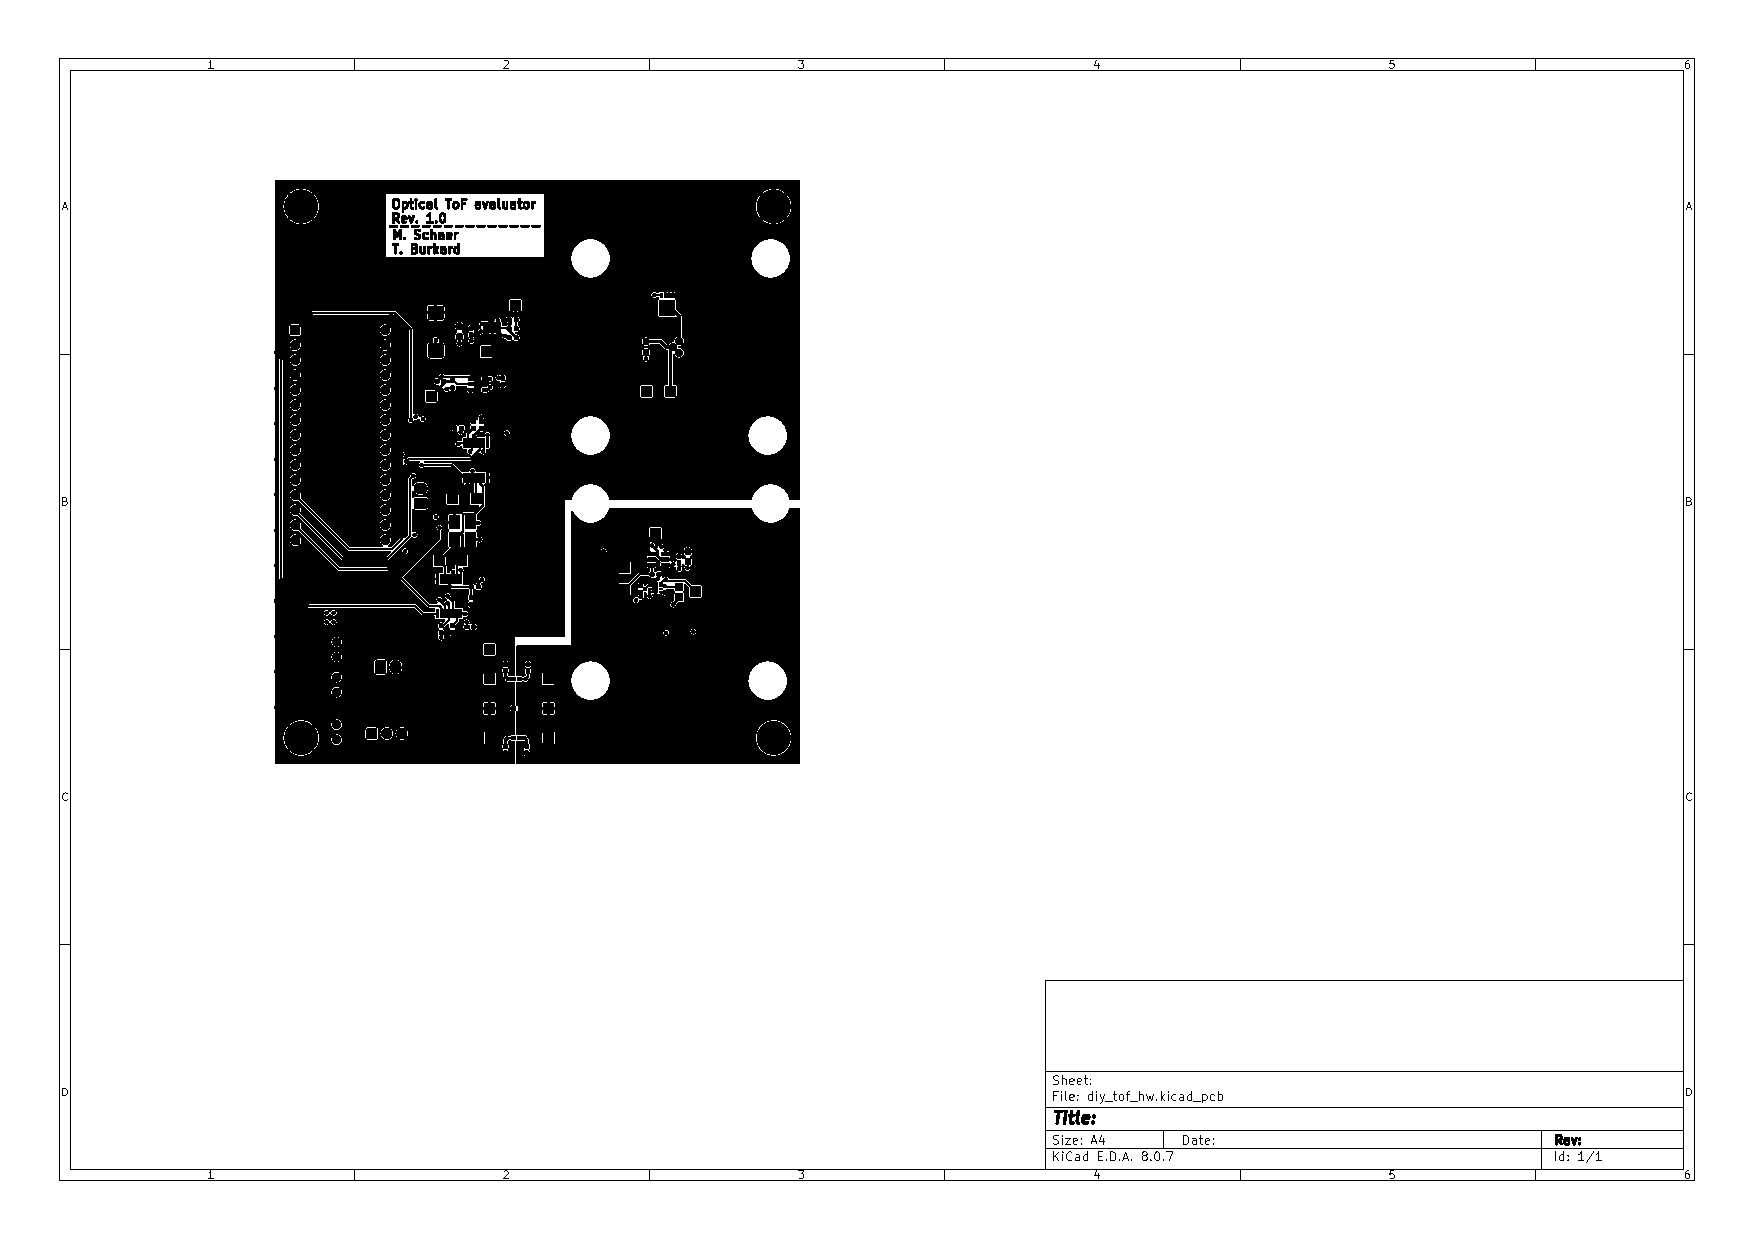
\includegraphics[trim=130 220 450 80, clip, width=0.6\textwidth]{attachments/pcb_F_Cu.pdf}
    \caption{PCB Layout Top}\label{fig:pcb_f_cu}
\end{figure}

\begin{figure}[H]
    \centering
    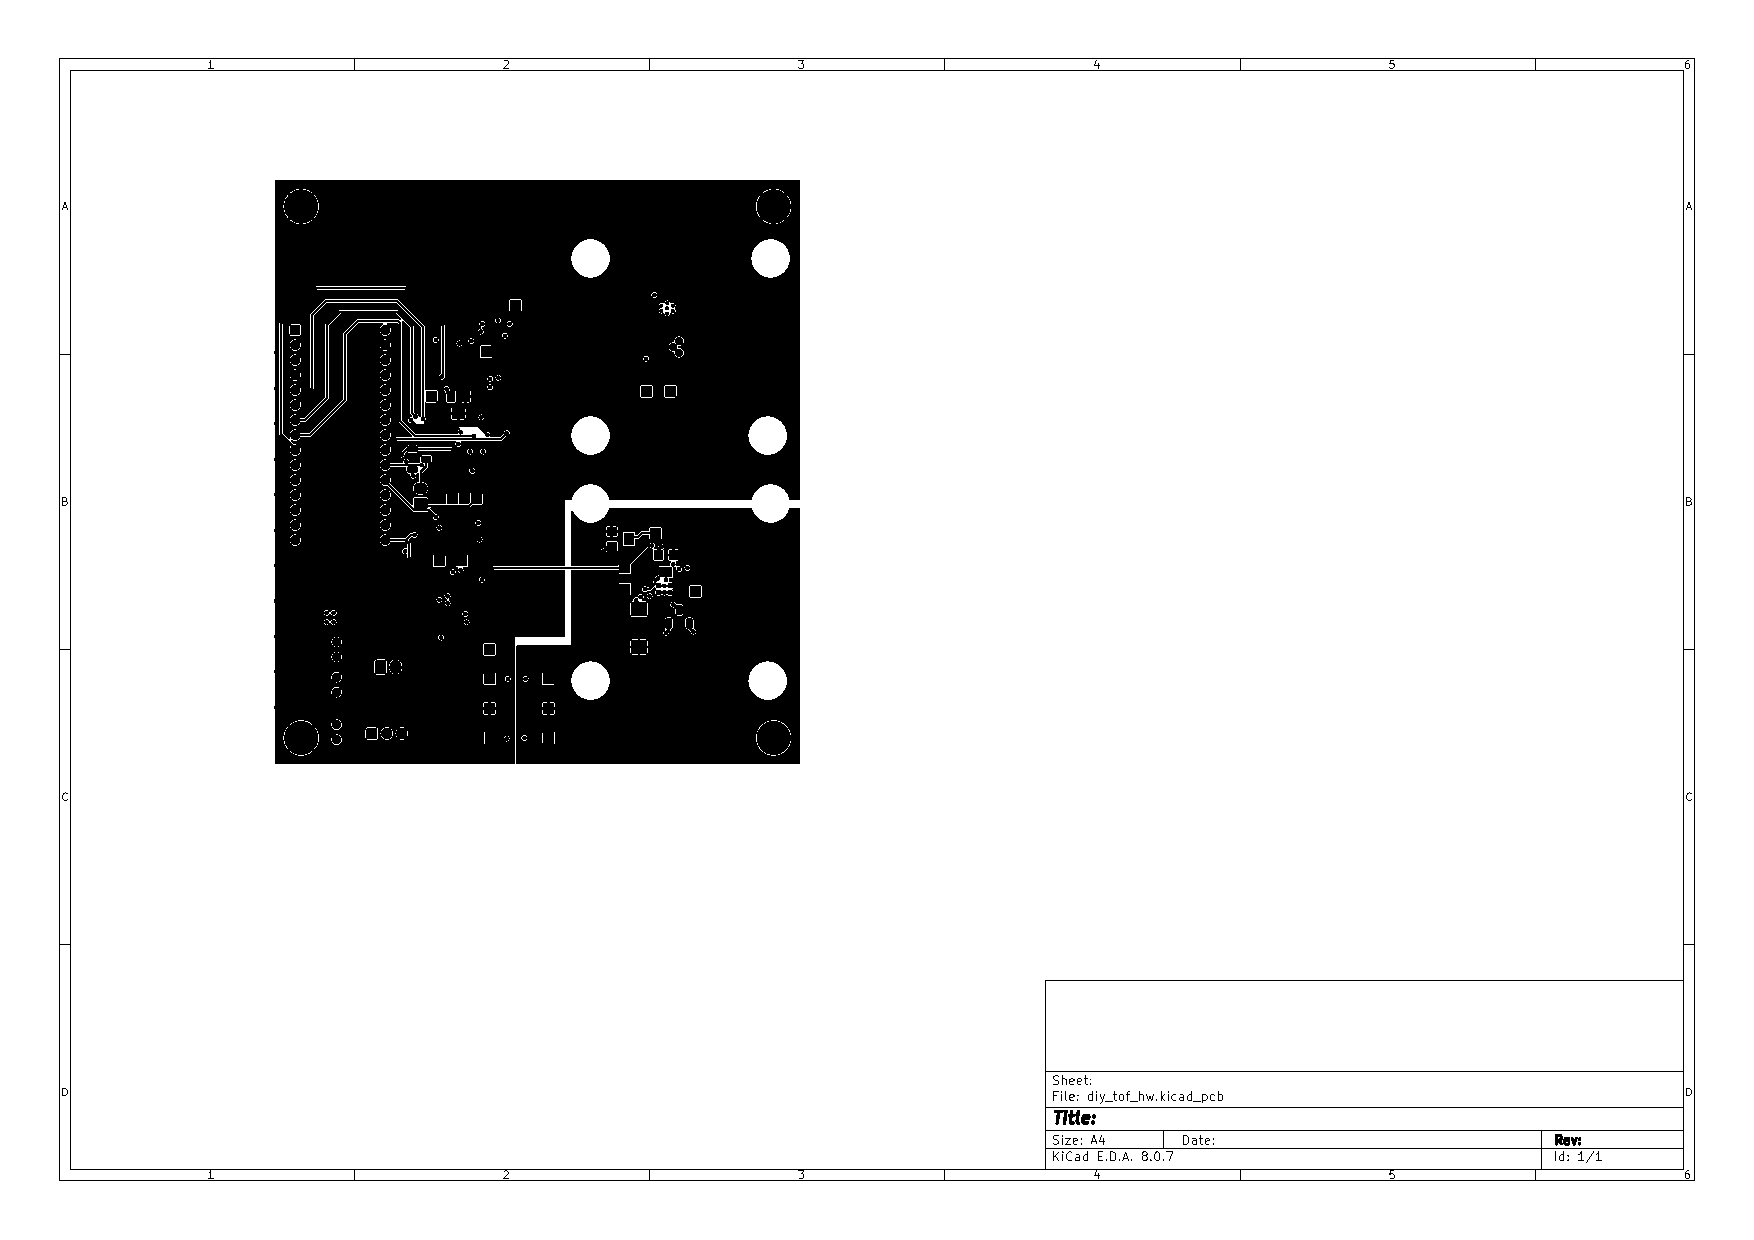
\includegraphics[trim=130 220 450 80, clip, width=0.6\textwidth]{attachments/pcb_B_Cu.pdf}
    \caption{PCB Layout Bottom}\label{fig:pcb_b_cu}
\end{figure}

\begin{figure}[H]
    \centering
    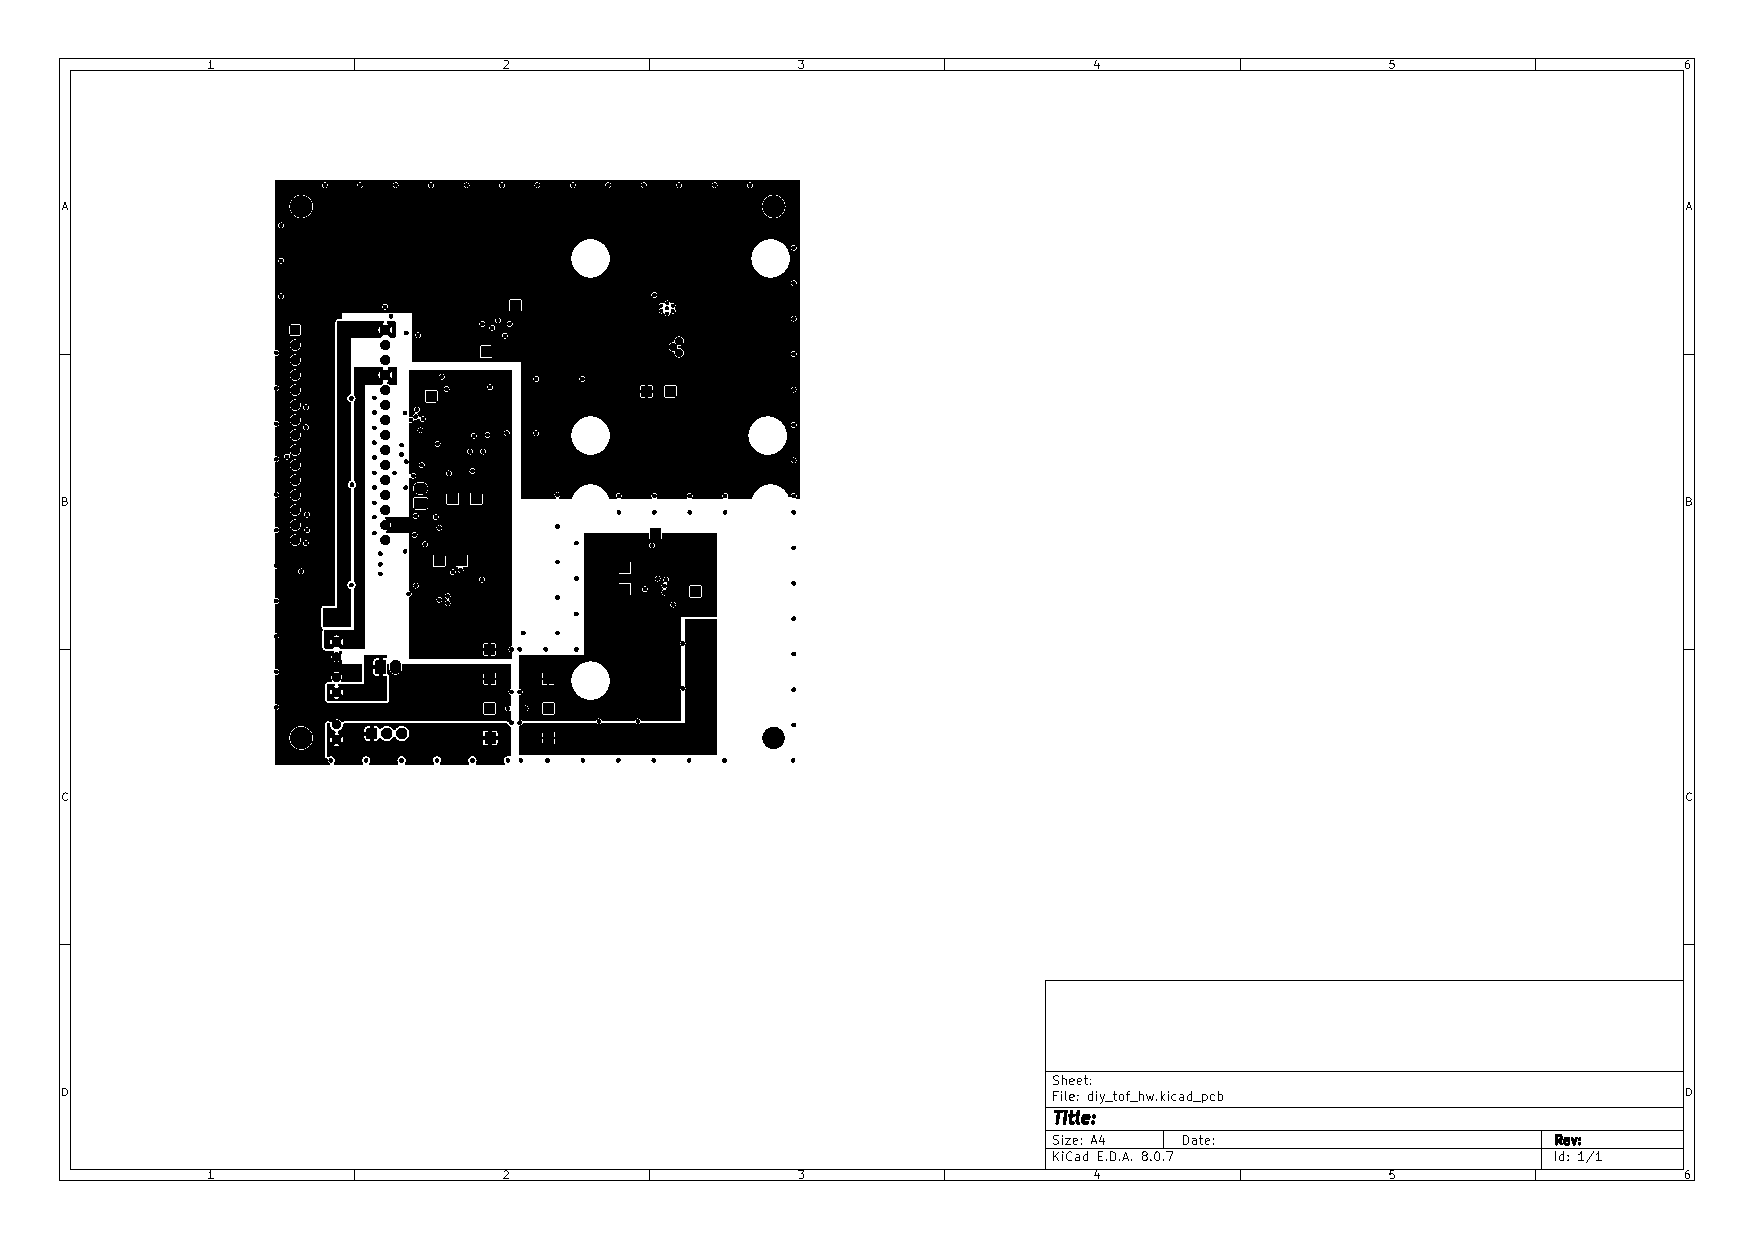
\includegraphics[trim=130 220 450 80, clip, width=0.6\textwidth]{attachments/pcb_In1_Cu.pdf}
    \caption{PCB Layout Innen 1}\label{fig:pcb_in1_cu}
\end{figure}

\begin{figure}[H]
    \centering
    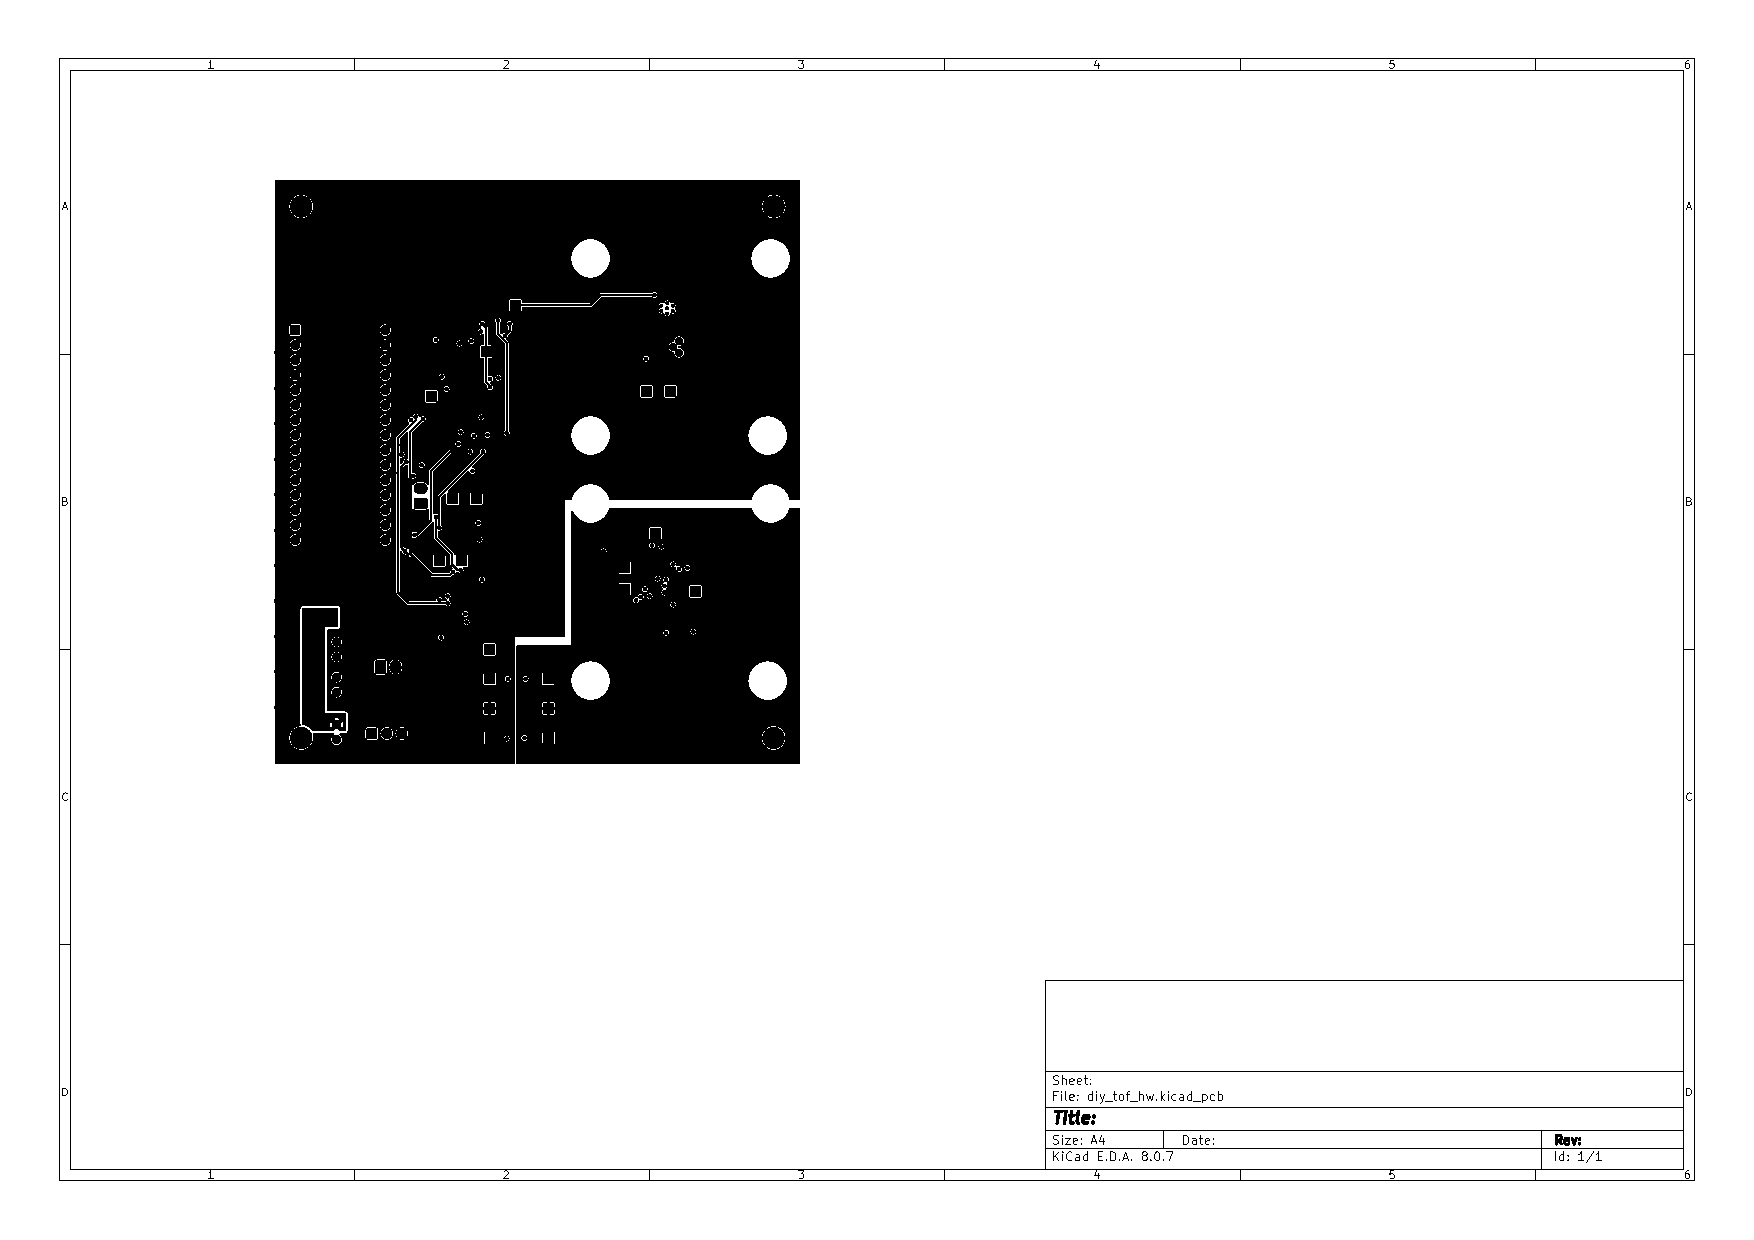
\includegraphics[trim=130 220 450 80, clip, width=0.6\textwidth]{attachments/pcb_In2_Cu.pdf}
    \caption{PCB Layout Innen 2}\label{fig:pcb_in2_cu}
\end{figure}

\subsubsection{Komponenten-Platzierung}

\begin{figure}[H]
    \centering
    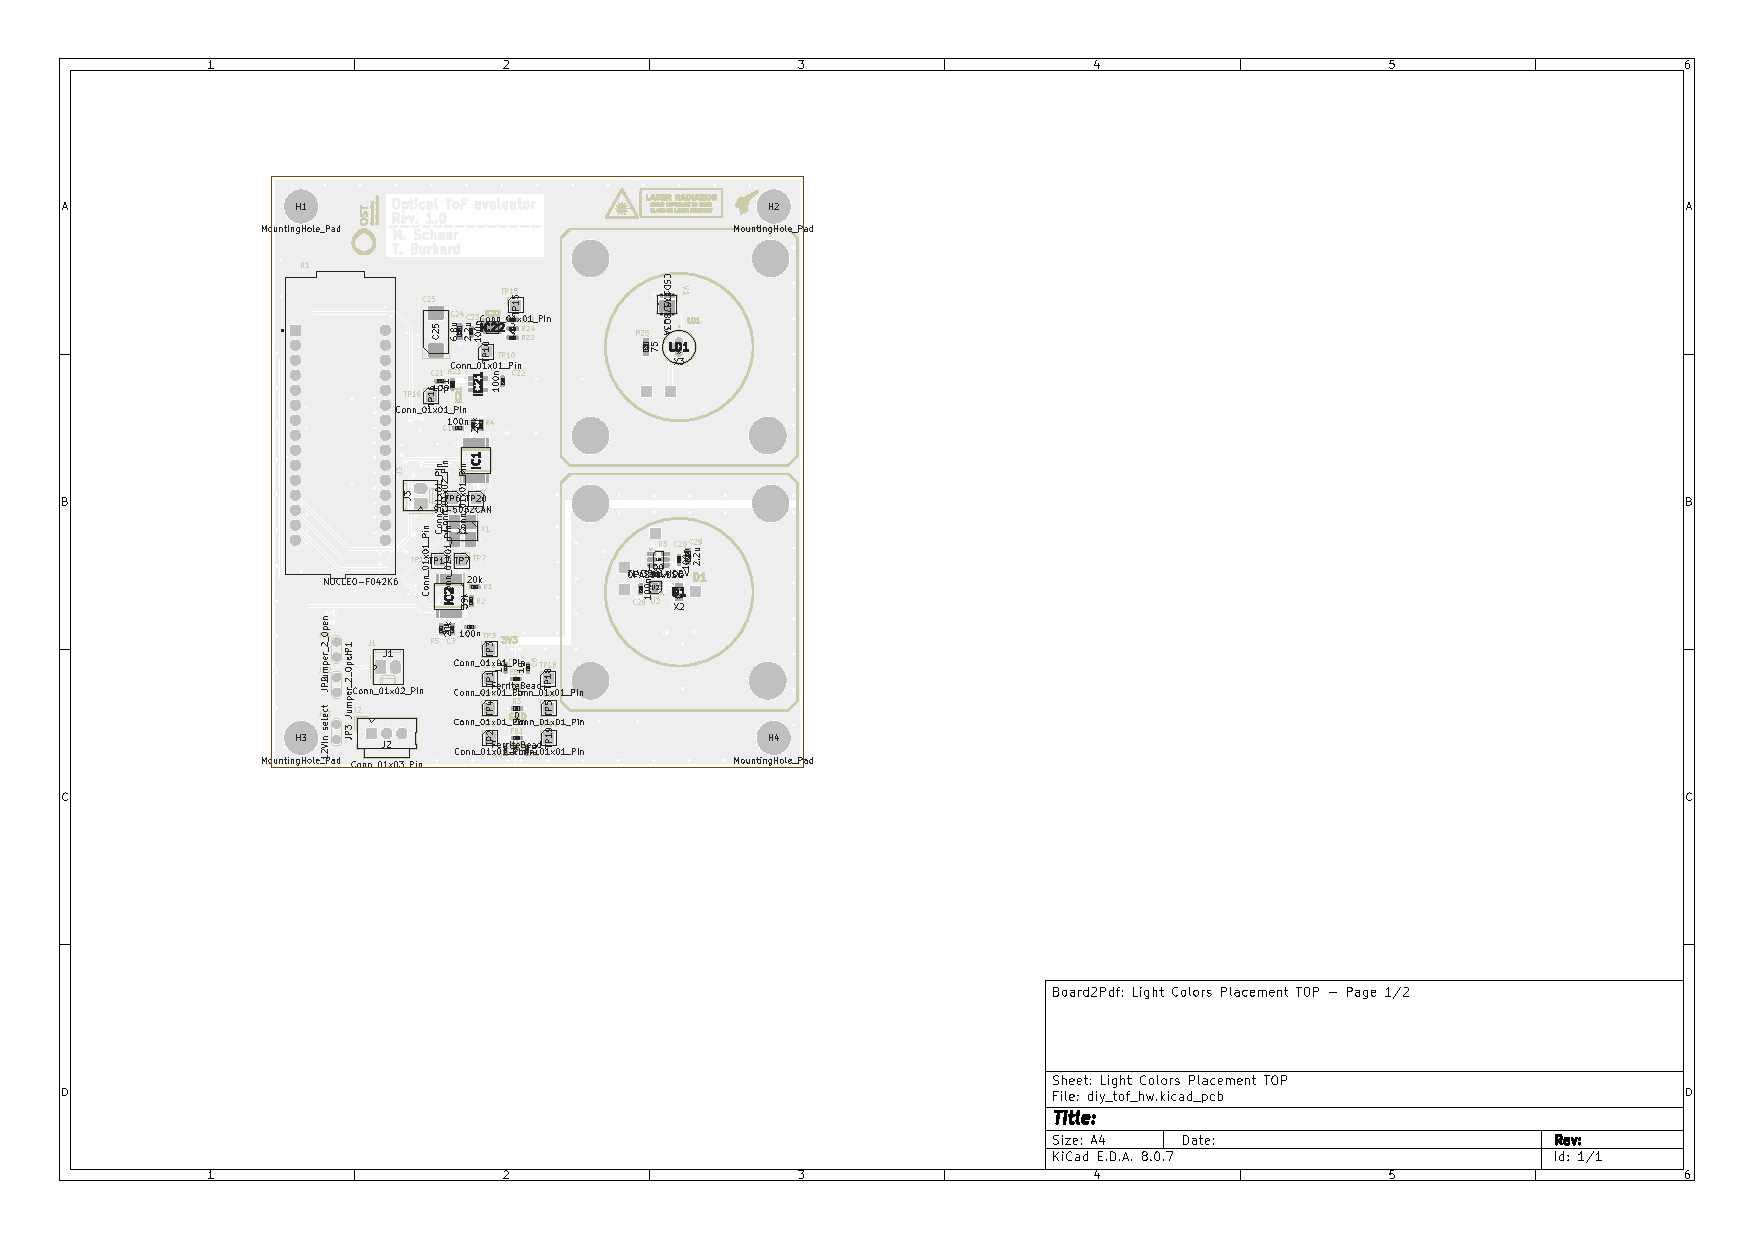
\includegraphics[page=1, trim=120 220 450 80, clip, width=0.6\textwidth]{attachments/pcb_placement.pdf}
    \caption{PCB Komponenten-Platzierung Top}\label{fig:pcb_placement_1}
\end{figure}

\begin{figure}[H]
    \centering
    \includegraphics[page=2, trim=450 220 120 80, clip, width=0.6\textwidth]{attachments/pcb_placement.pdf}
    \caption{PCB Komponenten-Platzierung Bottom}\label{fig:pcb_placement_2}
\end{figure}

\pagebreak

\subsection{3D View}

\begin{figure}[H]
    \centering
    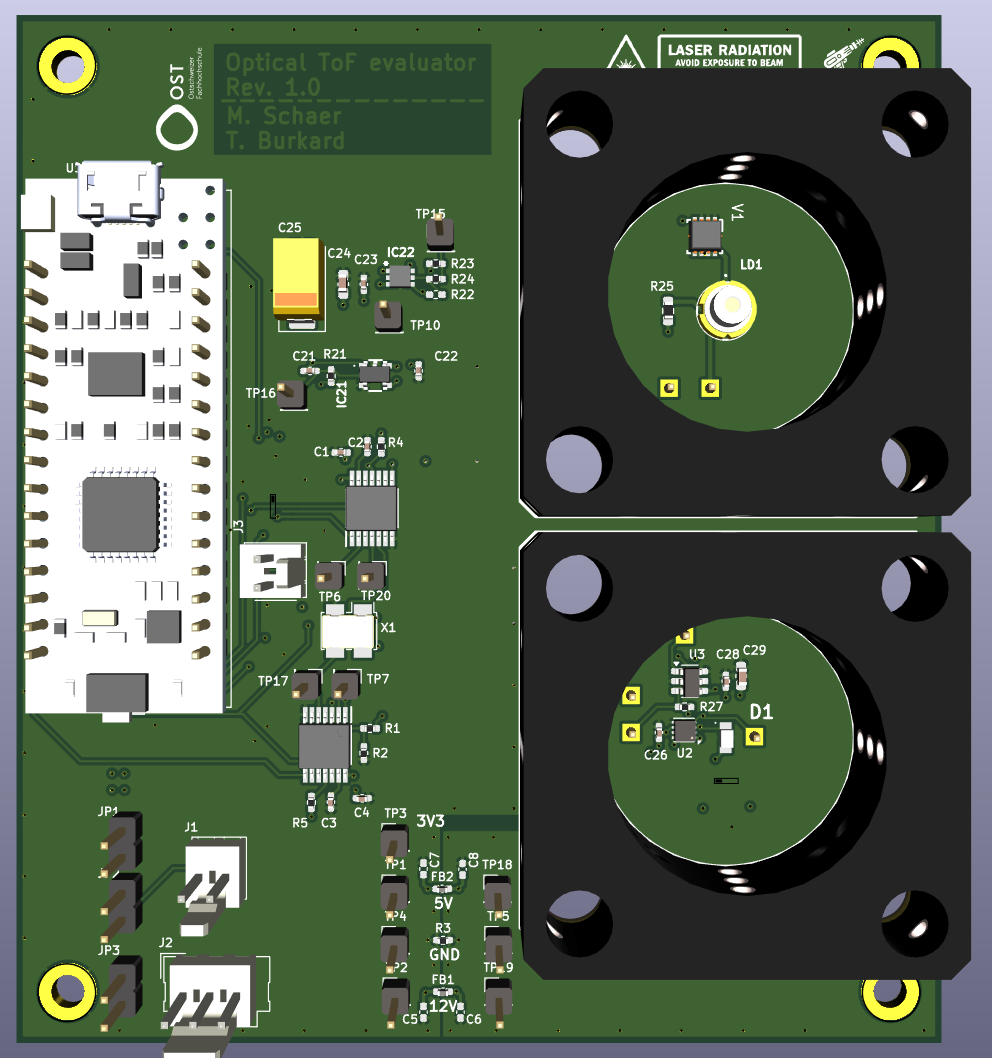
\includegraphics[width=0.6\textwidth]{graphics/3d_top.png}
    \caption{3D View Top}\label{fig:3d_top}
\end{figure}

\begin{figure}[H]
    \centering
    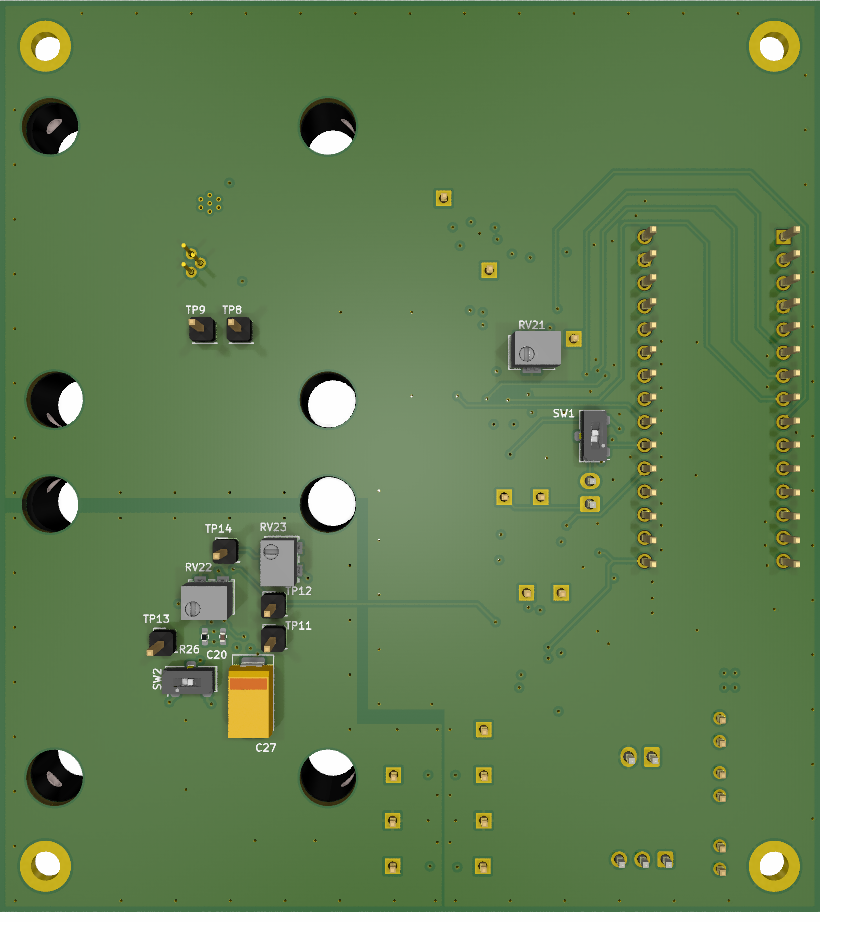
\includegraphics[width=0.6\textwidth]{graphics/3d_bottom.png}
    \caption{3D View Bottom}\label{fig:3d_bottom}
\end{figure}

\pagebreak

\section{Simulationen}

\subsection{Laser Treiber}
\subsection{Transimpedanzverstärker}

\pagebreak

\section{Messungen}

In diesem Kapitel werden die Messresultate dokumentiert.

Die verwendeten Python-Skripte zur Berechnung der statistischen Grössen und zum Plotten der Diagramme befinden sich im
Anhang Kapitel \ref{sec:python_analyze}.

Das verwendete \acrfull{dso} ist ein Rohde \& Schwarz RTB2004 1.25 GSa/s.

\subsection{Elektrische Messungen}

In diesem Teilkapitel werden die Messresultate dokumentiert, welche rein elektrisch (also ohne optischen Teil) erfasst
wurde.

Die Zeitmessungen werden von \lstinline|IC1| (siehe Abbildung~\ref{fig:tdc_ele_signal}) durchgeführt und von der
Firmware, welche auf dem Nucleo Board \lstinline|U1| (siehe Abbildung~\ref{fig:nucleo_board}) getriggert und ausgelesen.

\subsubsection{GPIO Toggle mit HAL}\label{sec:gpio_toggle_with_hal}

Als erstes wird gemessen, wie lange es für die \acrshort{cpu} der \acrshort{mcu} dauert mittels \acrfull{hal} - Library
\cite{st2020stm32f0_hal} zwei \acrshort{gpio}-Pins zu schalten.

In Code~\ref{code:gpio_toggle_with_hal} ist die Firmware-Implementation dazu gezeigt.

\lstinputlisting[language={C}, label={code:gpio_toggle_with_hal}, caption={\acrshort{gpio} Toggle mit \acrshort{hal}}]{sourcecode/gpio_toggle_with_hal.c}

Der \acrshort{tdc} misst also die Zeit zwischen Zeile 15 und 16 in Code~\ref{code:gpio_toggle_with_hal}. Dazu wird der
STOP-Pin des \acrshort{tdc} via \lstinline|SW1| mit \lstinline|stop_ele| verbunden. Der Kabelanschluss \lstinline|J3|
wird kurzgeschlossen. Siehe Abbildung~\ref{fig:tdc_ele_signal}.

Via \acrshort{uart} wurden 2000 Messwerte erfasst. Ein Ausschnitt davon ist in Code \ref{code:gpio_toggle_with_hal_log}
gezeigt. Die restlichen Daten befinden sich im elektronischen Anhang.

\lstinputlisting[language={}, label={code:gpio_toggle_with_hal_log}, caption={\acrshort{gpio} Toggle mit \acrshort{hal}}]{sourcecode/gpio_toggle_with_hal_log.txt}

Arithmetischer Mittelwert und Standardabweichung sind in Formel \ref{eq:gpio_toggle_with_hal} aufgeführt.

\begin{equation}\label{eq:gpio_toggle_with_hal}
    \begin{split}
        \overline{ToF} &= 6'375'888~ps\\
        \sigma         &= 1'059~ps
    \end{split}
\end{equation}
\myequations{\acrshort{gpio} Toggle mit \acrshort{hal}}

Da die \acrshort{cpu} mit 8~MHz läuft, lässt sich daraus schliessen, dass ein Pin-Toggle mit \acrshort{hal} ca. 50
\acrshort{cpu}-Cycles benötigt. Dies erscheint plausibel.

Histogramm und Boxplot sind in Abbildung~\ref{fig:gpio_toggle_with_hal_histogram} bzw.
\ref{fig:gpio_toggle_with_hal_boxplot} dargestellt.

\begin{figure}[H]
    \centering
    \includesvg[width=0.8\textwidth]{graphics/gpio_toggle_with_hal_histogram.svg}
    \caption{\acrshort{gpio} Toggle mit \acrshort{hal} - Histogramm}\label{fig:gpio_toggle_with_hal_histogram}
\end{figure}

\begin{figure}[H]
    \centering
    \includesvg[width=0.8\textwidth]{graphics/gpio_toggle_with_hal_boxplot.svg}
    \caption{\acrshort{gpio} Toggle mit \acrshort{hal} - Boxplot}\label{fig:gpio_toggle_with_hal_boxplot}
\end{figure}

Um die Resultate des \acrshort{tdc} zu validieren, wurde dieselbe Messung auch mittels \acrfull{dso} durchgeführt. Die
Messungen sind in Abbildung~\ref{fig:gpio_toggle_with_hal_dso} und \ref{fig:gpio_toggle_with_hal_dso_zoom} dargestellt.

\begin{figure}[H]
    \centering
    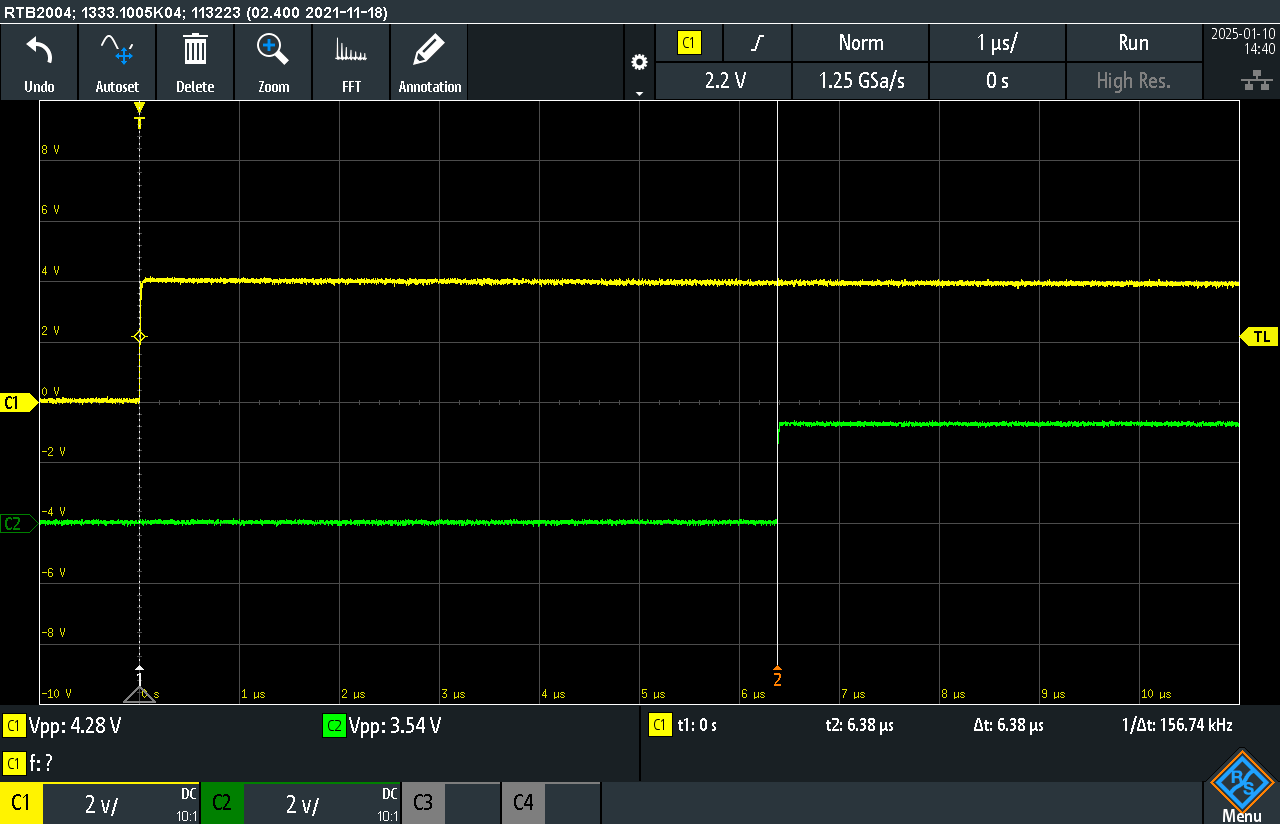
\includegraphics[width=0.8\textwidth]{graphics/gpio_toggle_with_hal_dso.png}
    \caption{\acrshort{gpio} Toggle mit \acrshort{hal} - \acrshort{dso}}\label{fig:gpio_toggle_with_hal_dso}
\end{figure}

\begin{figure}[H]
    \centering
    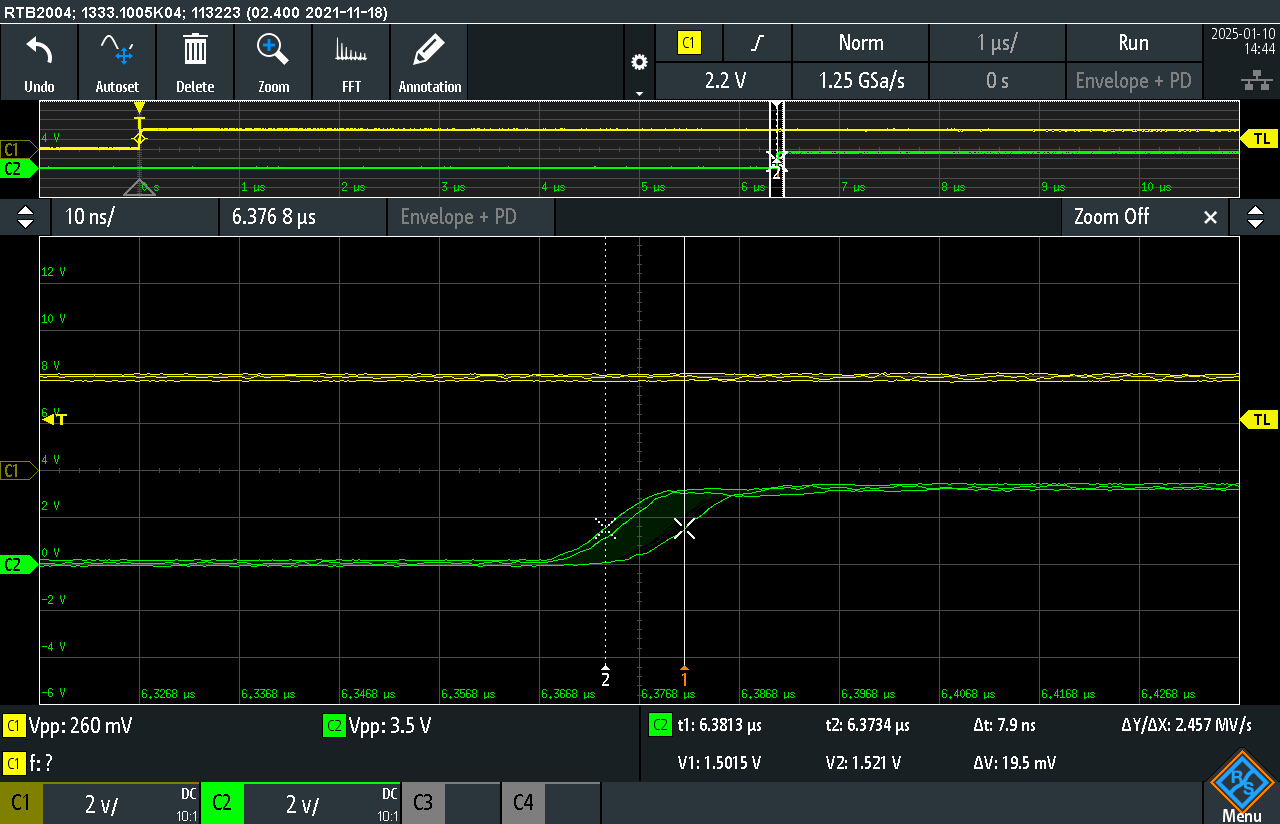
\includegraphics[width=0.8\textwidth]{graphics/gpio_toggle_with_hal_dso_zoom.png}
    \caption{\acrshort{gpio} Toggle mit \acrshort{hal} - \acrshort{dso} (Zoom)}\label{fig:gpio_toggle_with_hal_dso_zoom}
\end{figure}

\subsubsection{GPIO Toggle ohne HAL}\label{sec:gpio_toggle_without_hal}

Als nächstes wird gemessen wie lange es für die \acrshort{cpu} der \acrshort{mcu} dauert mit direktem Register-Zugriff
(via Pointer; ohne \acrshort{hal}-Library) zwei \acrshort{gpio}-Pins zu schalten.

In Code~\ref{code:gpio_toggle_without_hal} ist die Firmware-Implementation dazu gezeigt.

\lstinputlisting[language={C}, label={code:gpio_toggle_without_hal}, caption={\acrshort{gpio} Toggle ohne \acrshort{hal}}]{sourcecode/gpio_toggle_without_hal.c}

Der \acrshort{tdc} misst also die Zeit zwischen Zeile 15 und 16 in Code~\ref{code:gpio_toggle_without_hal}. Dazu wird,
wie in Kapitel \ref{sec:gpio_toggle_with_hal}, der STOP-Pin des \acrshort{tdc} via \lstinline|SW1| mit
\lstinline|stop_ele| verbunden. Der Kabelanschluss \lstinline|J3| wird kurzgeschlossen. Siehe
Abbildung~\ref{fig:tdc_ele_signal}.

Via \acrshort{uart} wurden 2000 Messwerte erfasst. Ein Ausschnitt davon ist in Code
\ref{code:gpio_toggle_without_hal_log} gezeigt. Die restlichen Daten befinden sich im elektronischen Anhang.

\lstinputlisting[language={}, label={code:gpio_toggle_without_hal_log}, caption={\acrshort{gpio} Toggle ohne \acrshort{hal}}]{sourcecode/gpio_toggle_without_hal_log.txt}

Arithmetischer Mittelwert und Standardabweichung sind in Formel \ref{eq:gpio_toggle_without_hal} aufgeführt.

\begin{equation}\label{eq:gpio_toggle_without_hal}
    \begin{split}
        \overline{ToF} &= 1'377'773~ps\\
        \sigma         &= 402~ps
    \end{split}
\end{equation}
\myequations{\acrshort{gpio} Toggle ohne \acrshort{hal}}

Da die \acrshort{cpu} mit 8~MHz läuft, lässt sich daraus schliessen, dass ein Pin-Toggle ohne \acrshort{hal} ca. 10
\acrshort{cpu}-Cycles benötigt. Dies erscheint plausibel.

Histogramm und Boxplot sind in Abbildung~\ref{fig:gpio_toggle_without_hal_histogram} bzw.
\ref{fig:gpio_toggle_without_hal_boxplot} dargestellt.

\begin{figure}[H]
    \centering
    \includesvg[width=0.8\textwidth]{graphics/gpio_toggle_without_hal_histogram.svg}
    \caption{\acrshort{gpio} Toggle ohne \acrshort{hal} - Histogramm}\label{fig:gpio_toggle_without_hal_histogram}
\end{figure}

\begin{figure}[H]
    \centering
    \includesvg[width=0.8\textwidth]{graphics/gpio_toggle_without_hal_boxplot.svg}
    \caption{\acrshort{gpio} Toggle ohne \acrshort{hal} - Boxplot}\label{fig:gpio_toggle_without_hal_boxplot}
\end{figure}

Um die Resultate des \acrshort{tdc} zu validieren, wurde dieselbe Messung auch mittels \acrfull{dso} durchgeführt. Die
Messungen sind in Abbildung~\ref{fig:gpio_toggle_without_hal_dso} und \ref{fig:gpio_toggle_without_hal_dso_zoom}
dargestellt.

\begin{figure}[H]
    \centering
    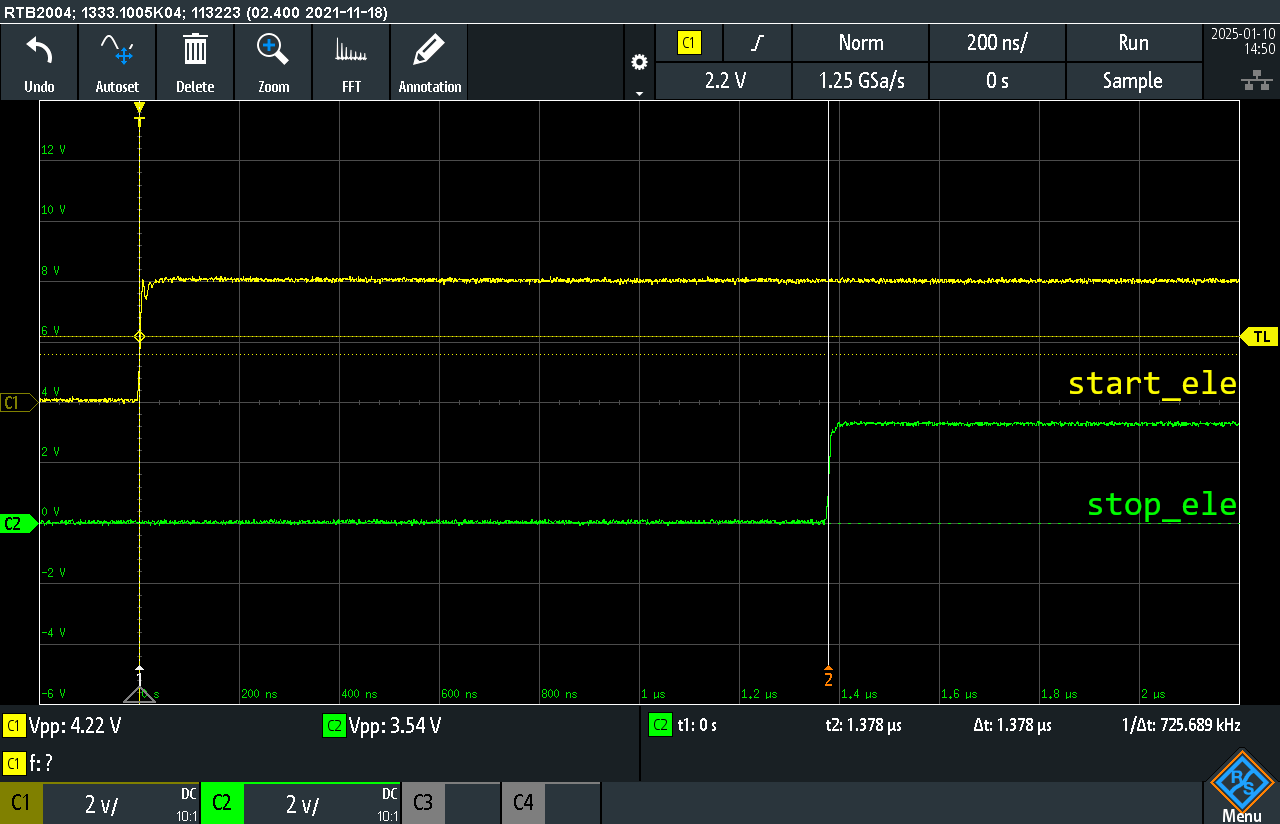
\includegraphics[width=0.8\textwidth]{graphics/gpio_toggle_without_hal_dso.png}
    \caption{\acrshort{gpio} Toggle ohne \acrshort{hal} - \acrshort{dso}}\label{fig:gpio_toggle_without_hal_dso}
\end{figure}

\begin{figure}[H]
    \centering
    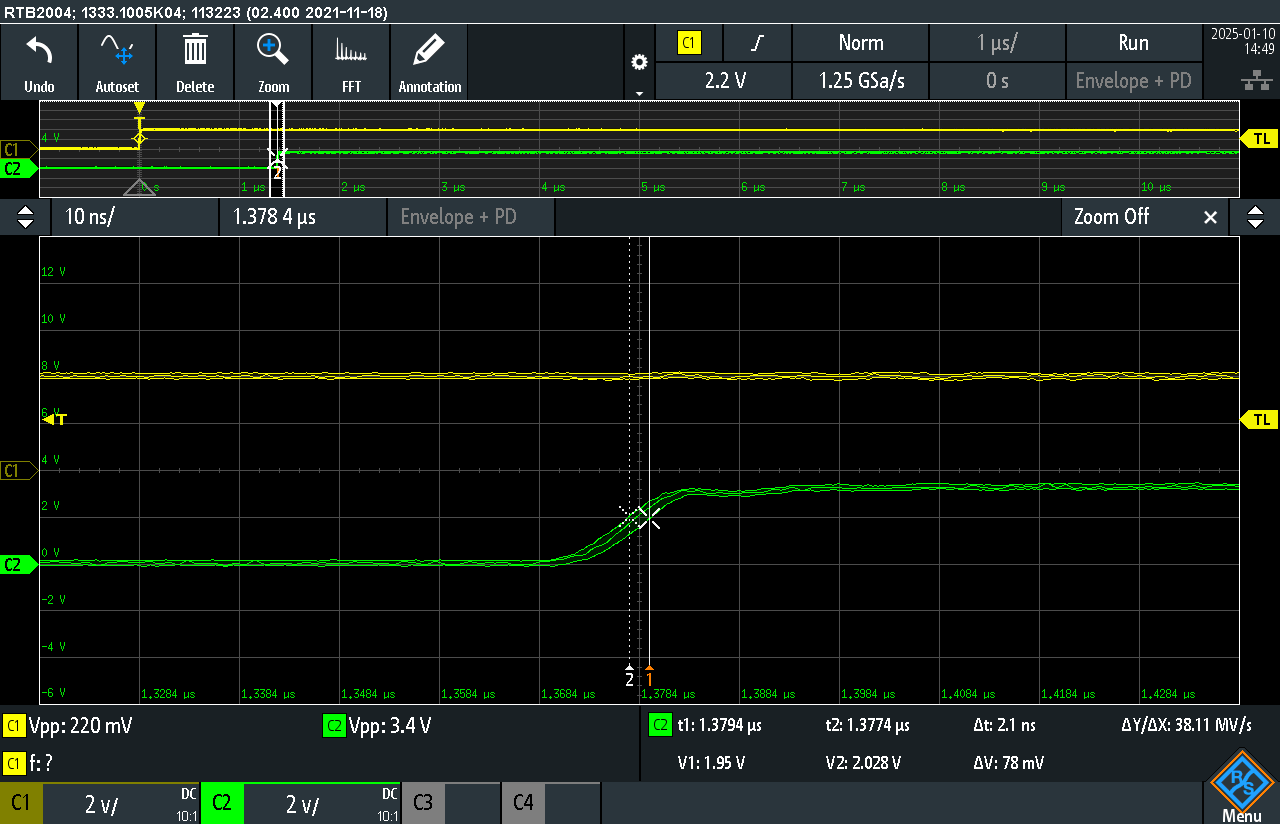
\includegraphics[width=0.8\textwidth]{graphics/gpio_toggle_without_hal_dso_zoom.png}
    \caption{\acrshort{gpio} Toggle ohne \acrshort{hal} - \acrshort{dso} (Zoom)}\label{fig:gpio_toggle_without_hal_dso_zoom}
\end{figure}

\subsubsection{Unterschiedliche Kabellängen}\label{sec:different_cable_lengths}

Für diese Messung wird dasselbe Setup wie in Kapitel \ref{sec:gpio_toggle_without_hal} verwendet.

Anstelle eines Kurzschlusses von \lstinline|J3| (siehe Abbildung \ref{fig:tdc_ele_signal}) werden nun verschiedene
Kabellängen angeschlossen.

Es hat sich herausgestellt, dass eine kreisförmige Anordnung des Kabels wichtig ist. Denn bei einer Überlappung der
beiden Kabelenden werden kürze Zeiten gemessen. Dies hat mit der kapazitiven Kopplung zwischen den Leitern zu tun.

Die Resultate sind in Abbildung~\ref{fig:different_cable_lengths} dargestellt. Die Liste mit den Datenpunkten befindet
sich im elektronischen Anhang.

\begin{figure}[H]
    \centering
    \includesvg[width=0.9\textwidth]{graphics/different_cable_lengths.svg}
    \caption{Unterschiedliche Kabellängen}\label{fig:different_cable_lengths}
\end{figure}

Die arithmetischen Mittelwerte und Standardabweichungen sind in Tabelle \ref{tab:different_cable_lengths} aufgeführt.

\begin{table}[H]
    \mytable
        {|l|l|l|}
        {\textbf{Länge} & \textbf{Mittelwert} & \textbf{Standardabweichung}}
        {\length & \mean & \stddev}
        {tables/different_cable_lengths.csv}
    \caption{Unterschiedliche Kabellängen}\label{tab:different_cable_lengths}
\end{table}

Die Signal-Ausbreitungsgeschwindigkeit in Kupfer beträgt ca. 2/3 der Lichtgeschwindigkeit
\cite{firewallcx2025propagationdelay}. Um die Resultate in Tabelle \ref{tab:different_cable_lengths} zu validieren,
rechnen wir wie in Formel \ref{eq:cable_length} gezeigt, auf die Kabellänge zurück. Die Laufzeit bei 0~m wird dabei
abgezogen, um die Verzögerung zu kompensieren, welche durch das Schalten der \acrshort{gpio}s entsteht.

\begin{equation}\label{eq:cable_length}
    \begin{split}
        c_{cu} &\approx \frac{2}{3} \cdot c_0 = \frac{2}{3} \cdot 299'792'458~\frac{m}{s} \approx 200'000'000~\frac{m}{s}\\
        ToF_{n} &= ToF_{n_{abs}} - ToF_{0}\\
        l_{n}   &= ToF_{n} \cdot c_{cu}
    \end{split}
\end{equation}
\myequations{Zurückrechnen auf Kabellänge}

Die Resultate sind in Tabelle \ref{tab:different_cable_lengths_calc} dargestellt.

\begin{table}[H]
    \mytable
        {|l|l|l|}
        {\textbf{Tatsächliche Länge} & \textbf{ToF\_n} & \textbf{Zurückgerechnete Länge}}
        {\reallength & \tofn & \calclength}
        {tables/different_cable_lengths_calc.csv}
    \caption{Kabellängen zurückgerechnet}\label{tab:different_cable_lengths_calc}
\end{table}

Es fällt auf, dass die Resultate nicht genau übereinstimmen. Dies hat mehrere Ursachen: Die Ausbreitungsgeschwindigkeit
ist nicht genau bekannt und die tatsächlichen Kabellängen wurden nicht genau gemessen.

%TODO Lets challenge this. Maybe 2/3 c is wrong for pure copper and it should be something like 95\% ?

Es ist jedoch eine klare Korrelation zu erkennen.

\subsubsection{Mode 1 vs. Mode 2}

%TODO: Evtl. Beschreibung der TDC-Modi in ein anderes Kapitel verschieben. z.B. Theorie/TDC?

Der \acrshort{tdc}7200 unterstützt zwei Modi mit unterschiedlichen Messbereichen \cite{ti2016tdc7200_datasheet}:

\begin{itemize}
    \item Mode 1: 12~ns bis 500~ns
    \item Mode 2: 250~ns bis 8~ms
\end{itemize}

Im Mode~1 wird nur der interne Ring-Oszillator des \acrshort{tdc} verwendet. Siehe dazu Abbildung~\ref{fig:tdc_mode1}.

\begin{figure}[H]
    \centering
    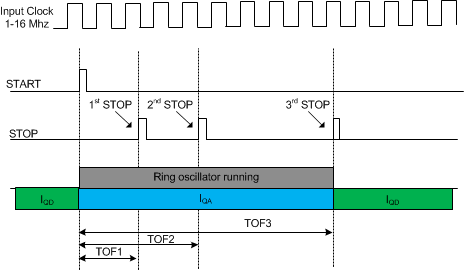
\includegraphics[width=0.6\textwidth]{graphics/tdc_mode1.png}
    \caption[\acrshort{tdc} Mode 1]{\acrshort{tdc} Mode 1 \cite{ti2016tdc7200_datasheet}}\label{fig:tdc_mode1}
\end{figure}

Im Mode~2, um längere Zeiten messen zu können, wir zusätzlich der externe Clock des \acrshort{tdc} verwendet. Siehe dazu
Abbildung~\ref{fig:tdc_mode2}.

\begin{figure}[H]
    \centering
    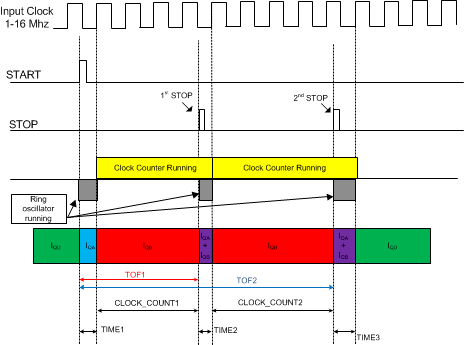
\includegraphics[width=0.6\textwidth]{graphics/tdc_mode2.png}
    \caption[\acrshort{tdc} Mode 2]{\acrshort{tdc} Mode 2 \cite{ti2016tdc7200_datasheet}}\label{fig:tdc_mode2}
\end{figure}

Die bisherigen Messungen (Kapitel~\ref{sec:gpio_toggle_with_hal}, \ref{sec:gpio_toggle_without_hal} und
\ref{sec:different_cable_lengths}) wurden im Mode~2 durchgeführt, da das Schalten der \acrshort{gpio}s mit der
\acrshort{cpu} mehr als 500~ns brauchte.

In künftigen Messungen soll das Schalten der \acrshort{gpio}s von einem Hardware-Timer der \acrshort{mcu} erledigt
werden. Damit werden Schaltzeiten von 125~ns bei 8~MHz bzw. 20.8~ns bei 48~MHz möglich sein. Es soll deshalb in diesem
Kapitel ein Vergleich der Messresultate der beiden Modi gemacht werden.

Dazu wurden drei Messungen gemacht:
\begin{enumerate}
    \item \acrshort{gpio} Toggle ohne \acrshort{hal} im Mode~2 mit Kabellänge~=~0~m (wie in Kapitel~\ref{sec:gpio_toggle_without_hal} und \ref{sec:different_cable_lengths})
    \item \acrshort{gpio} Toggle ohne \acrshort{hal} im Mode~2 mit Kabellänge~=~6~m (wie in Kapitel~\ref{sec:different_cable_lengths})
    \item Ohne GPIO Toggle Im Mode~1 mit Kabellänge~=~6~m
\end{enumerate}

Für die Messung im Mode~1 soll auf die Verzögerung durch das Schalten der \acrshort{gpio}s verzichtet werden. Dazu wird
das Start- und Stop-Signal vom selben \acrshort{gpio}-Pin, \lstinline|START_ELE|, generiert. Dazu wird \lstinline|SW1|
mit \lstinline|start_ele| verbunden (siehe Abbildung~\ref{fig:tdc_ele_signal}).

In Code~\ref{code:mode1} ist die Firmware-Implementation für eine Messung im Mode~1 gezeigt.

\lstinputlisting[language={C}, label={code:mode1}, caption={Mode 1}]{sourcecode/mode1.c}

Die Unterschiede im Vergleich zu den Messungen in Kapitel~\ref{sec:gpio_toggle_without_hal} und
\ref{sec:different_cable_lengths} sind:

\begin{itemize}
    \item Zeile 7: \acrshort{tdc} wird im Mode~1 konfiguriert (anstatt Mode~2)
    \item Zeile 15 und 23: Es wird nur der \lstinline|START_ELE| Pin getoggelt (anstatt \lstinline|START_ELE| und \lstinline|STOP_ELE| Pin)
\end{itemize}

Die Erwartung ist, dass die Differenz aus Messung~1 und Messungen~2 ungefähr dem Resultat aus Messung~3 entspricht.

Die Resultate dieser drei Messungen sind in Tabelle \ref{tab:mode1_vs_mode2} aufgeführt. Die restlichen Daten befinden
sich im elektronischen Anhang.

\begin{table}[H]
    \mytable
        {|l|l|l|}
        {\textbf{Messung} & \textbf{Mittelwert} & \textbf{Standardabweichung}}
        {\measurement & \mean & \stddev}
        {tables/mode1_vs_mode2.csv}
    \caption{Mode 1 vs. Mode 2}\label{tab:mode1_vs_mode2}
\end{table}

Die Berechnung in Formel~\ref{eq:mode1_vs_mode2} zeigt, dass die Messresultate nahe beieinander liegen.

\begin{equation}\label{eq:mode1_vs_mode2}
    \begin{split}
        \Delta Mode~2 &= 1'403'224~ps - 1'378'222~ps = 25'001~ps\\
        Mode~1        &= 25'145~ps
    \end{split}
\end{equation}
\myequations{Mode 1 vs. Mode 2}

Es kann also davon ausgegangen werden, dass Mode~1 und Mode~2 im Firmware-Treiber korrekt implementiert wurden.

Bemerkung: Im Firmware-Treiber (siehe Anhang Kapitel \ref{sec:tdc_driver}) kann für beide Modi dieselbe Funktion
\lstinline|TDC_read_result()| verwendet werden. Für Mode~1 vereinfacht sich die Berechnung, weil \lstinline|TIME2|~=~0
und \lstinline|CLOCK_COUNT1|~=~0.

\subsubsection{Timer Output}\label{sec:timer_output}

In Kapitel~\ref{sec:gpio_toggle_with_hal} und \ref{sec:gpio_toggle_without_hal} wurge gezeigt, dass es einige
\acrshort{cpu}-Cycles dauert, um  mittels Software, also mit \acrshort{cpu}-Instruktionen, \acrshort{gpio}s zu toggeln.

Eine schnellere Methode ist es, das Toggeln der \acrshort{gpio}s von der Hardware-Peripherie der \acrshort{mcu}
erledigen zu lassen. Dazu eignen sich Hardware-Timer.

In Abbildung \ref{fig:clock_config_default} ist die default Clock-Configuration des Nucleo-Boards gezeigt.

\begin{figure}[H]
    \centering
    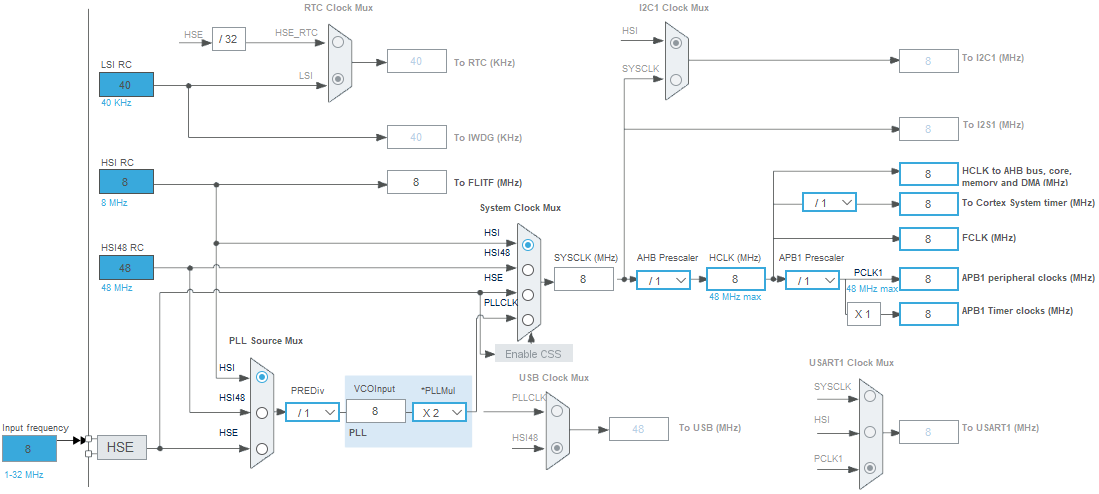
\includegraphics[width=0.9\textwidth]{graphics/clock_config_default.png}
    \caption{Default Clock-Configuration}\label{fig:clock_config_default}
\end{figure}

Per default wir der \acrfull{hsi} Clock mit 8~MHz verwendet. Damit sollte es mit Hardware-Timer möglich sein, zwei
\acrshort{gpio}s zu schalten mit einer Verzögerung von 1~/~8~MHz = 125~ns.

Dazu werden Kanal \lstinline|CH1| und \lstinline|CH4| des Hardware-Timers \lstinline|TIM1| im Output Compare Match Modus
verwendet. Die zugeordneten \acrshort{gpio}-Pins sind \lstinline|start_ele| bzw. \lstinline|stop_ele|.

Erreicht der 16bit-Timer den Wert \lstinline|32'000| wird \lstinline|start_ele| auf High geschalten. Beim Erreichen des
Werts \lstinline|32'001| wird \lstinline|stop_ele| auf High geschalten.

Der \acrshort{tdc} wird in Mode 1 konfiguriert. Der STOP-Pin des \acrshort{tdc} wird via \lstinline|SW1| mit
\lstinline|stop_ele| verbunden. Der Kabelanschluss \lstinline|J3| wird kurzgeschlossen. Siehe
Abbildung~\ref{fig:tdc_ele_signal}.

In Code~\ref{code:timer_output} ist die Firmware-Implementation dazu gezeigt.

\lstinputlisting[language={C}, label={code:timer_output}, caption={\acrshort{gpio} Toggle mit Timer-Output}]{sourcecode/timer_output.c}

Der gemessene arithmetische Mittelwert und die Standardabweichung sind in Formel~\ref{eq:timer_output} aufgeführt.  Die
Liste mit den Datenpunkten befindet sich im elektronischen Anhang.

\begin{equation}\label{eq:timer_output}
    \begin{split}
        \overline{ToF} &=128'108~ps\\
        \sigma         &= 81~ps
    \end{split}
\end{equation}
\myequations{\acrshort{gpio} Toggle mit Timer-Output}

Erwartungsgemäss dauert das Schalten der \acrshort{gpio}s ca. 125~ns. Die Standardabweichung ist aufgrund der kleineren
Anzahl an Clock-Cycles tiefer als in den bisherigen Kapiteln.

\subsubsection{Unterschiedliche Clock-Konfigurationen}

In diesem Teilkapitel werden Messungen mit demselben Setup wie in Kapitel~\ref{sec:timer_output} durchgeführt.

Es werden die arithmetischen Mittelwerte und die Standardabweichungen verschiedener Clock-Quellen des Nucleo-Boards
verglichen. Es werden drei Messungen gemacht:

\begin{enumerate}
    \item \acrshort{hsi}: 8~MHz (wie in Kapitel~\ref{sec:timer_output})
    \item \acrshort{hsi} mit \acrshort{pll}: 16~MHz
    \item \acrshort{hsi}48: 48~MHz
\end{enumerate}

Die Clock-Konfigurationen für Messung 2 und 3 sind in Abbildung~\ref{fig:clock_config_hsi_pll_16mhz} bzw.
\ref{fig:clock_config_hsi48_48mhz} dargestellt.

\begin{figure}[H]
    \centering
    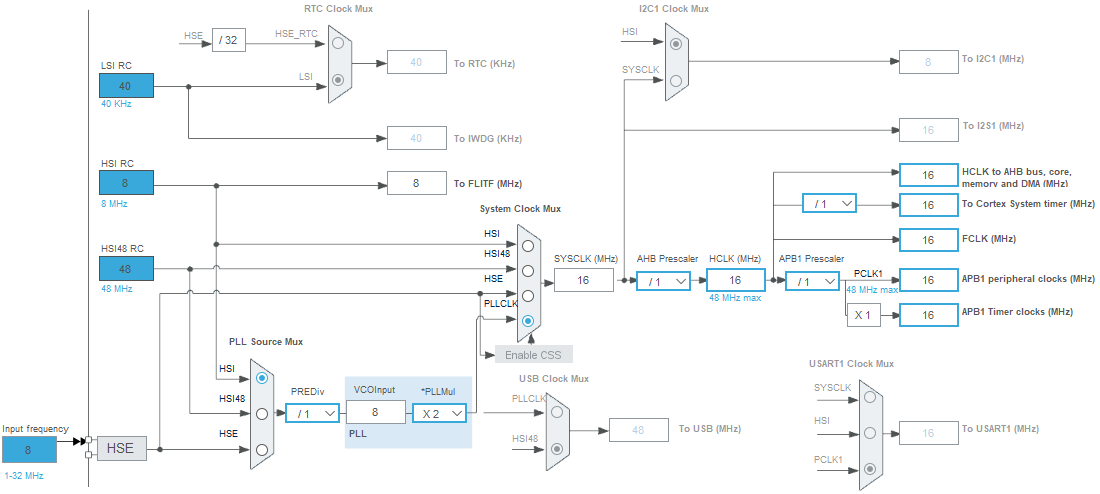
\includegraphics[width=0.9\textwidth]{graphics/clock_config_hsi_pll_16mhz.png}
    \caption{Clock-Configuration \acrshort{hsi} mit \acrshort{pll} 16~MHz}\label{fig:clock_config_hsi_pll_16mhz}
\end{figure}

\begin{figure}[H]
    \centering
    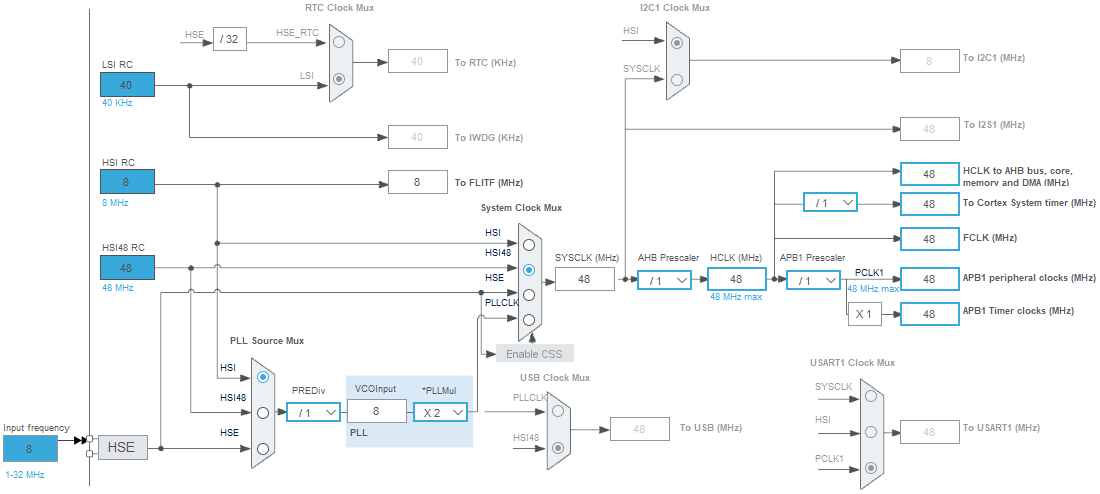
\includegraphics[width=0.9\textwidth]{graphics/clock_config_hsi48_48mhz.png}
    \caption{Clock-Configuration \acrshort{hsi}48 48~MHz}\label{fig:clock_config_hsi48_48mhz}
\end{figure}

Die arithmetischen Mittelwerte und Standardabweichungen sind in Tabelle~\ref{tab:different_clock_sources} dargestellt.
Die Liste mit den Datenpunkten befindet sich im elektronischen Anhang.

\begin{table}[H]
    \mytable
        {|l|l|l|}
        {\textbf{Messung} & \textbf{Mittelwert} & \textbf{Standardabweichung}}
        {\measurement & \mean & \stddev}
        {tables/different_clock_sources.csv}
    \caption{Unterschiedliche Clock-Quellen}\label{tab:different_clock_sources}
\end{table}

Die Resultate stimmen ungefähr mit den erwarteten Werten von 1~/~8~MHz = 125~ns, 1~/~16~MHz = 62.5~ns und
1~/~48~MHz = 20.8~ns überein.

Im Datenblatt konnte eine Angabe zum \acrshort{pll}-Jitter gefunden werden, siehe Abbildung~\ref{fig:pll_jitter}.

\begin{figure}[H]
    \centering
    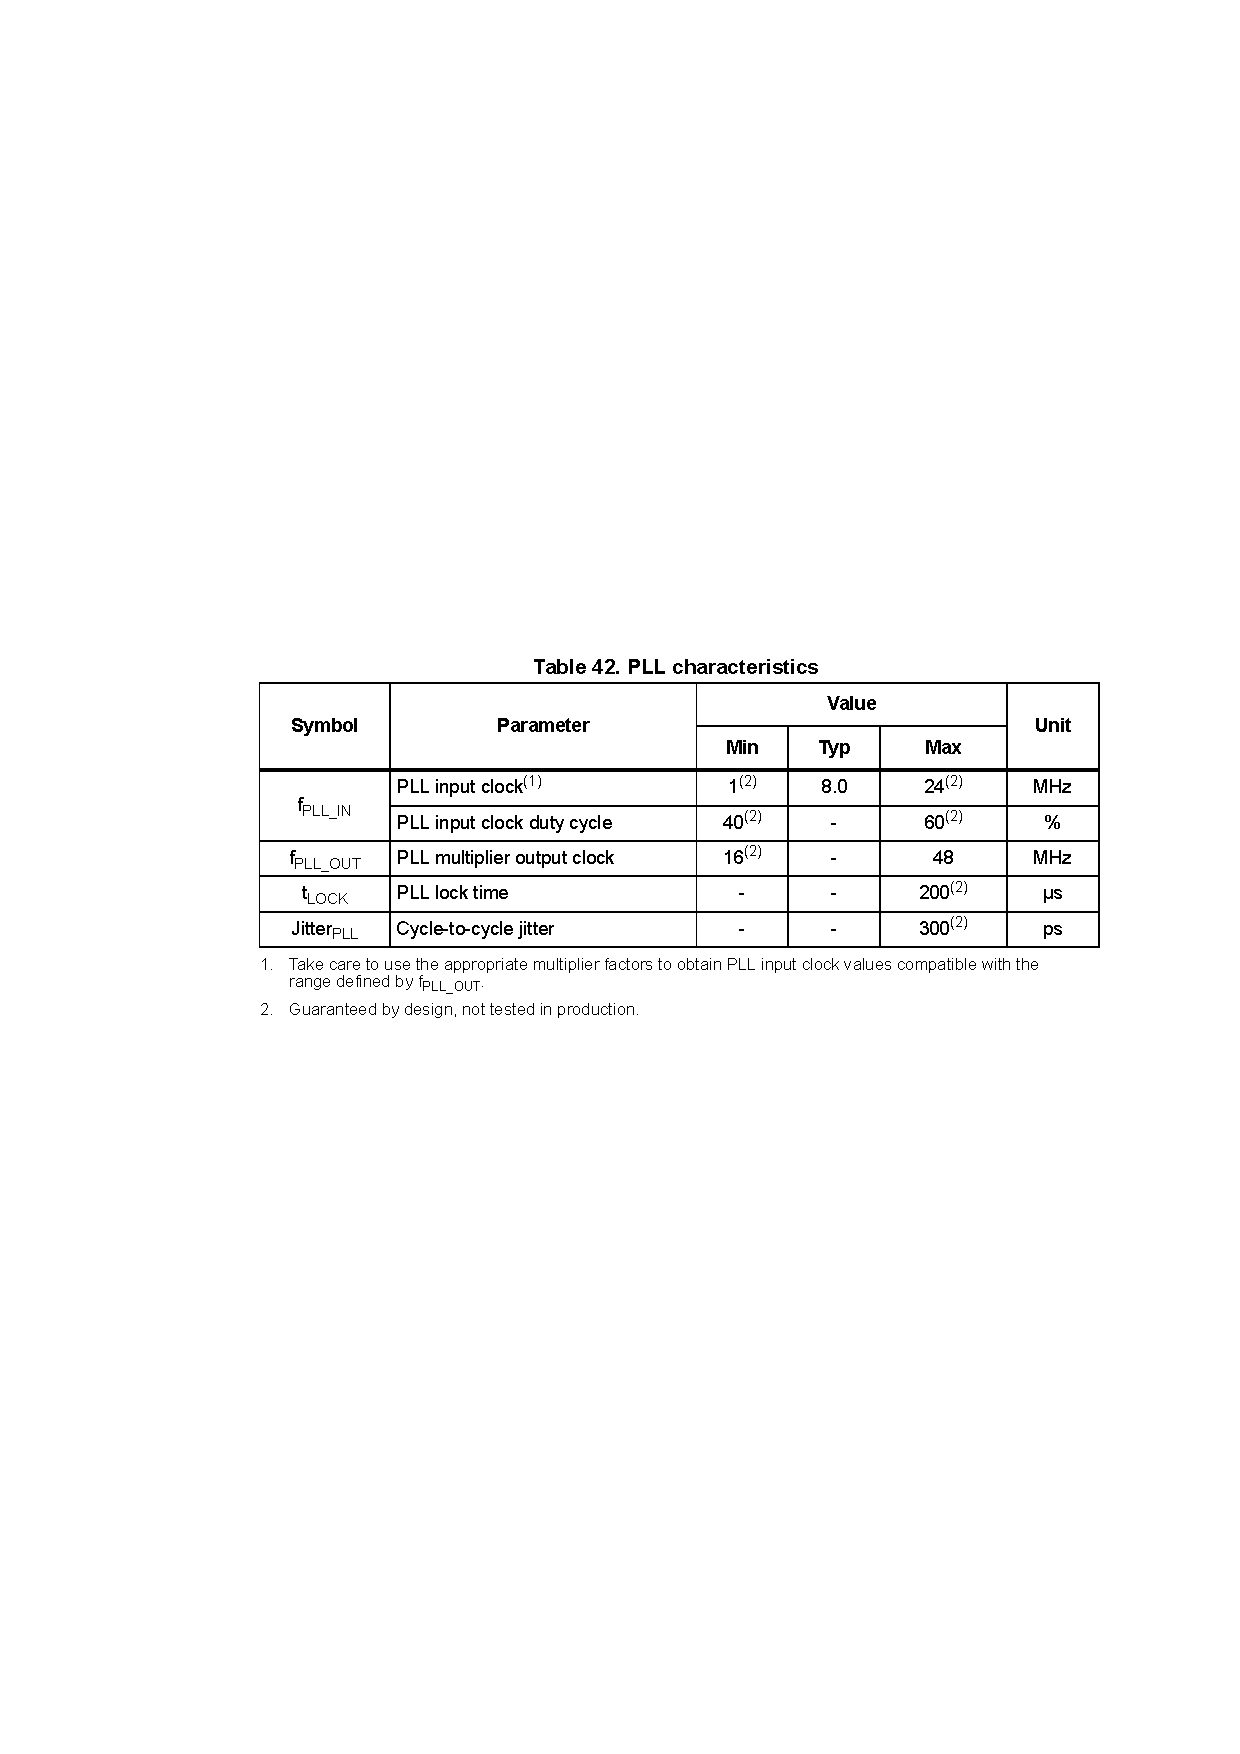
\includegraphics[width=0.8\textwidth]{graphics/pll_jitter.pdf}
    \caption[\acrshort{pll}-Jitter]{\acrshort{pll}-Jitter \cite{st2017stm32f042k6_datasheet}}\label{fig:pll_jitter}
\end{figure}

Diese Angabe ist ungefähr in derselben Grössenordnung wie die Messresultate.

\pagebreak

\subsection{Optische Messungen}

%TODO

\pagebreak

\section{Fazit}

\pagebreak

\section{Anhang}

\subsection{TDC Treiber}\label{sec:tdc_driver}

In Code~\ref{code:tdc_driver_header} und \ref{code:tdc_driver_source} ist der selbst entwickelte Firmware-Treiber für
den \acrshort{tdc} dargestellt.

\lstinputlisting[language={c}, label={code:tdc_driver_header}, caption={TDC Driver (Header)}]{../firmware/Core/TDC/TDC.h}
\lstinputlisting[language={c}, label={code:tdc_driver_source}, caption={TDC Driver (Source)}]{../firmware/Core/TDC/TDC.c}

\subsection{Python Analyse}\label{sec:python_analyze}

In Code \ref{code:python_analyze} ist das Python-Skript zur Berechnung des arithmetischen Mittelwerts und der
Standardabweichung sowie zum Plotten des Histogramms und des Boxplots dargestellt.

\lstinputlisting[language={python}, label={code:python_analyze}, caption={Python Analyse}]{../utilities/analyze-tof.py}

In Code \ref{code:python_analyze_multi} ist das Python-Skript zur Berechnung des arithmetischen Mittelwerts und der
Standardabweichung sowie zum Plotten der Werte für mehrere Messungen dargestellt.

\lstinputlisting[language={python}, label={code:python_analyze_multi}, caption={Python Analyse (Multi)}]{../utilities/analyze-tofs.py}
\pagebreak

\begin{landscape}

    \subsection{Schema}\label{sec:schematic_apdx}
    \global\pdfpageattr\expandafter{\the\pdfpageattr/Rotate 90}
    \begin{figure}[H]
        \centering
        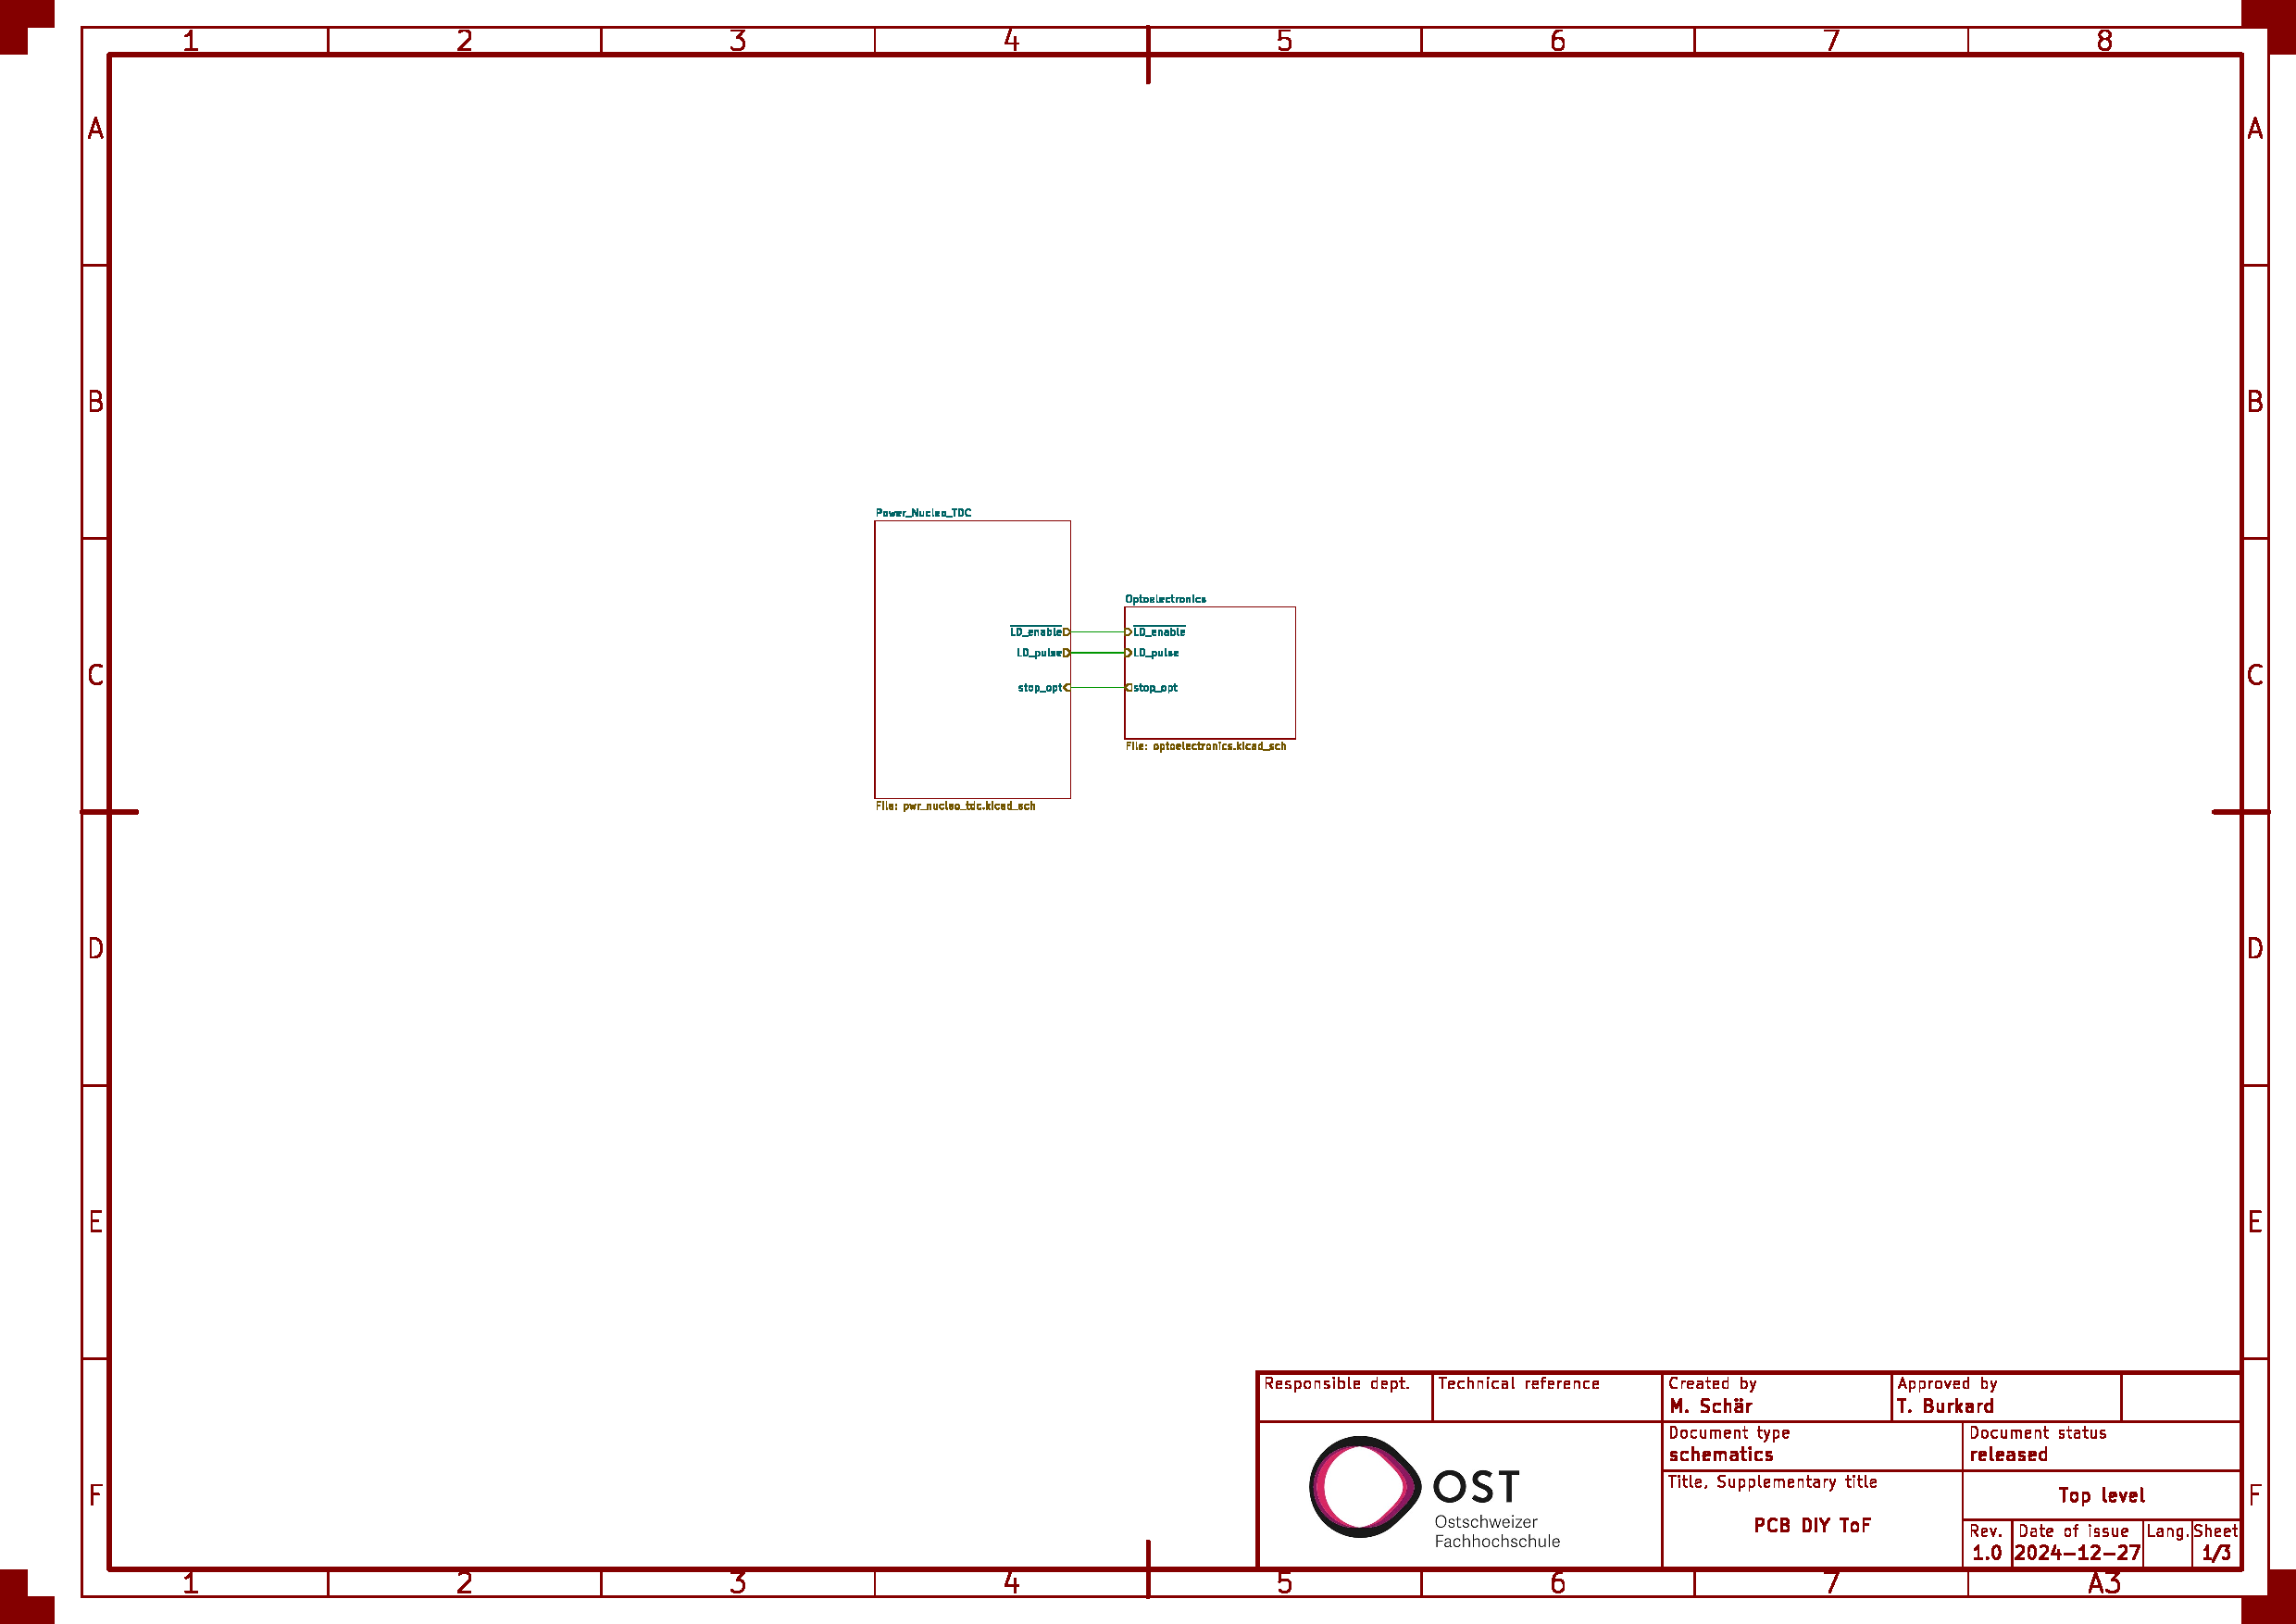
\includegraphics[page=1, width=1.2\textwidth]{attachments/schematic.pdf}
        \caption{Schema S.1/3}\label{fig:schematics_1}
    \end{figure}
    \pagebreak

    \global\pdfpageattr\expandafter{\the\pdfpageattr/Rotate 90}
    \begin{figure}[H]
        \centering
        \includegraphics[page=2, width=1.2\textwidth]{attachments/schematic.pdf}
        \caption{Schema S.2/3}\label{fig:schematics_2}
    \end{figure}
    \pagebreak

    \global\pdfpageattr\expandafter{\the\pdfpageattr/Rotate 90}
    \begin{figure}[H]
        \centering
        \includegraphics[page=3, width=1.2\textwidth]{attachments/schematic.pdf}
        \caption{Schema S.3/3}\label{fig:schematics_3}
    \end{figure}
    \pagebreak


    \subsection{Stückliste}

    \begin{table}[H]
        \scriptsize
        \mytable
            {|l|l|l|l|l|l|}
            {\textbf{Reference} & \textbf{Value} & \textbf{Datasheet} & \textbf{Footprint} & \textbf{Qty} & \textbf{DNP}}
            {\Reference & \Value & \Datasheet & \Footprint & \Qty & \DNP}
            {tables/bom.csv}
        \caption{Bill of Material}\label{tab:bom}
    \end{table}

\end{landscape}

\global\pdfpageattr\expandafter{\the\pdfpageattr/Rotate 0}
%%%%%%%%%%%%%%%%%%%%%% CONTENT END %%%%%%%%%%%%%%%%%%%%%%

\pagebreak

\section*{Quellenverzeichnis}
\begin{flushleft}
\begingroup
\vspace{-25pt}
\renewcommand\refname{}
\renewcommand{\addcontentsline}[3]{} % Do not add bibliography to table of contents, as there is a separate subsection "Quellenverzeichnis"
\bibliography{references}
\endgroup
\end{flushleft}


\end{document}
